\documentclass[12pt]{report}
\usepackage[format=plain,
            font=it]{caption}
%====================== PACKAGES ======================
%Options: Sonny, Lenny, Glenn, Conny, Rejne, Bjarne, Bjornstrup
% \usepackage{csquotes}
\usepackage[Glenn]{fncychap} 
\usepackage{fancyhdr}
\usepackage[final]{pdfpages}
\usepackage{algorithm}
\usepackage{algpseudocode}
\usepackage[utf8]{inputenc}
\usepackage[english]{babel}
%pour gérer les positionnement d'images
\usepackage{float}
\usepackage[sorting=none]{biblatex}
\usepackage{graphicx}
\usepackage[colorinlistoftodos]{todonotes}
\usepackage{url}
\renewcommand{\contentsname}{Table of Contents}
\usepackage{enumitem}
% this is for numbering and showing (subsubsections) in the toc
\setcounter{secnumdepth}{3}
\setcounter{tocdepth}{3}
%pour la mise en page des tableaux
\usepackage{array}
\usepackage{tabularx}
\usepackage{dcolumn,ragged2e}
\usepackage{siunitx}
\usepackage{longtable}
\usepackage{booktabs}   
\usepackage{ltablex}
\newcolumntype{L}{>{\raggedright\arraybackslash}X}
%pour utiliser \floatbarrier
\usepackage{colortbl}
%espacement entre les lignes
\usepackage{setspace}
%modifier la mise en page de l'abstract
\usepackage{abstract}
%police et mise en page (marges) du document
\usepackage[T1]{fontenc}
\usepackage[a4paper, top=2.5cm, bottom=2.5cm, left=2.5cm, right=2.5cm]{geometry}
\usepackage{amsmath,amsfonts,amssymb}
%Pour les galerie d'images
\usepackage{makecell}
\usepackage{multirow}
%\usepackage{subfig}
\usepackage{amsthm}
\newtheorem{definition}{Définition}
\usepackage{rotating}
%\usepackage{multirow}
\usepackage{xspace}
\usepackage{wrapfig}
\usepackage[hypertexnames=false]{hyperref}
\hypersetup{
    colorlinks=true,
    linkcolor=black,
    filecolor=black,      
    urlcolor=black,
    anchorcolor=black,
    citecolor=blue,
}
\usepackage{subcaption}
\usepackage{tablefootnote}
\usepackage[acronym]{glossaries}
\newcommand{\HRule}{\rule{\linewidth}{0.5mm}}
\addbibresource{citation.bib}
\begin{document} 
%%d'ici aussi
\begin{titlepage}   
    	\begin{minipage}{1\linewidth}
			\centering
			\begin{tabular}{ccc}
				\begin{tabular}{c}
					\\
					\includegraphics[scale=0.07]{figures/usthb.png}
				\end{tabular}
				&
				\begin{tabular}{c}
					\\
					\text{ République Algérienne Démocratique et Populaire}\\
                    \text{ Ministère de l’Enseignement Supérieur et de la Recherche} \\
                    \text{ Scientifique}\\
				\end{tabular}
				&
				\begin{tabular}{c}
					\\
					\includegraphics[scale=0.07]{figures/usthb.png}
				\end{tabular}
			\end{tabular}
		\end{minipage}
    
    
       
    \begin{center}
        
        \textbf{Université des Sciences et de la Technologie Houari Boumediene}\\
        \text{Faculté d’Électronique et d’Informatique}\\
        \text{Département d’Informatique}\\
        \textbf{Mémoire de Master}\\
        \text{Spécialité :}\\
        \text{Bio-informatique}\\
        
        
    \end{center}
    \vspace*{0.5 cm}
    \begin{center}
    
    \end{center}
    
    \rule{\linewidth}{0.2 mm}
	{ \LARGE  
	   \begin{center}
	       \textbf{Thème: }\\
	       \textbf{Optimising federated learning for healthcare applications}\\
	       
	   \end{center} 
	   
	\rule{\linewidth}{0.2 mm} \\[1.5 cm]
	}
	
	\begin{minipage}{0.5\textwidth}
		\begin{flushleft} \large
		    \textbf{Encadré par:}\\
		    \text{Mme Malika MEHDI-SILHADI}\\
		    \text{Mme MEKAHLIA}\\
		    \textbf{Membre du Jurys:}\\
		    \text{NOM Prenom}\\
		    \text{NOM Prenom}\\
		    
			\end{flushleft}
			\end{minipage}~
		\begin{minipage}{0.4\textwidth}
            
		\begin{flushright} \large
			\textbf{Présenté par:} \\
            \text{TALEB Youcef} \\
            \text{BENSEFIA Yazid} \\
            	\textbf{Soutenu le:} \\
            \text{18/09/2022} \\
		\end{flushright}
	\end{minipage}\\[2 cm]
	\begin{center}
	    Projet:  SII\_E\_0XX / 2026
	\end{center}
\end{titlepage}
%changing names%
\renewcommand{\listfigurename}{Listes des figures}
\renewcommand{\listtablename}{Listes des tableaux}

% \include{Chapters/remerciements}
% % ============================================================
%  resume.tex — Résumé en français
% ============================================================
\chapter*{Résumé}
\addcontentsline{toc}{chapter}{Résumé}

La classification des sous-types moléculaires du cancer
du sein à partir de l'IRM dynamique avec contraste
(DCE-IRM) est une tâche cliniquement importante~: le
sous-type détermine si une patiente peut bénéficier d'une
hormonothérapie ou nécessite une chimiothérapie.
L'entraînement d'un classifieur automatique se heurte
cependant à plusieurs obstacles concrets~: un seul hôpital
dispose rarement de plus de 800 patientes, le déséquilibre
entre sous-types atteint 10~pour~1, et les réglementations
de protection des données --- dont la loi algérienne 18-07
--- empêchent les institutions de regrouper leurs archives
d'imagerie.

Ce travail étudie si l'apprentissage fédéré peut produire
un classifieur utile dans ce contexte, sans qu'aucune
donnée patient ne quitte son institution d'origine.
L'étude est menée sur une cohorte publique de 737~patients
(Hôpital Duke, Zenodo DOI~10.5281/zenodo.7956360) avec
quatre sous-types~: Luminal~A, Luminal~B, HER2-enrichi
et Triple-Négatif.

Un pipeline d'entraînement local en trois étapes a été
construit à partir de composants éprouvés dans la
littérature~: un backbone ConvNeXt-Nano avec apprentissage
multi-instance à attention gated (MIL) traite les volumes
entiers sans masques de segmentation~; la perte LDAM,
l'optimisation ASAM, la moyenne de poids stochastique
(SWA) et le réentraînement du classifieur (cRT) corrigent
le déséquilibre de classe à chaque étape.
Ce pipeline atteint un macro~F1 de~0,342 (quatre classes)
et 0,667 (binaire) sur le pli de validation.

Pour l'expérience fédérée, trois clients hospitaliers
simulés sont construits selon une partition de Dirichlet
($\alpha = 0{,}5$).
FedAvg s'effondre vers la classe majoritaire
(macro~F1~= 0,429).
L'algorithme proposé FedSCRT --- qui combine un backbone
SCAFFOLD et un réentraînement fédéré du classifieur avec
échantillonnage équilibré --- atteint un macro~F1 de~0,629
et un AUC de~0,687, comblant 84,1~\% de l'écart de
performance fédérée et dépassant l'AUC de référence
centralisée.
Un résultat théorique montre que l'échantillonnage équilibré
rend le gradient du classifieur indépendant de la
distribution locale des classes, et une expérience contrôlée
de similarité cosinus sur trois hôpitaux artificiels le
confirme~: les gradients équilibrés s'alignent sur l'objectif
global ($\cos \geq 0,99$) quel que soit le préalable local,
tandis que les gradients naturels dérivent vers la classe
majoritaire, expliquant la robustesse de l'étape de
réentraînement fédéré du classifieur face à l'hétérogénéité
des distributions hospitalières.

\vspace{1em}
\noindent\textbf{Mots-clés~:} Apprentissage fédéré,
IRM mammaire, classification moléculaire, déséquilibre
de classes, FedSCRT, MIL à attention gated, LDAM,
SCAFFOLD.

% % ============================================================
%  abstract.tex — English Abstract
% ============================================================
\chapter*{Abstract}
\addcontentsline{toc}{chapter}{Abstract}

Breast cancer molecular subtype classification from
Dynamic Contrast-Enhanced MRI (DCE-MRI) is a clinically
important task: the subtype determines whether a patient
is eligible for hormone therapy or requires chemotherapy.
Training an automated classifier is, however, difficult
in practice.
A single hospital typically holds fewer than 800 patients,
the class imbalance between subtypes reaches 10:1, and
data protection regulations --- including Algerian Law
18-07 --- prevent institutions from pooling their imaging
archives.

This work investigates whether federated learning can
produce a useful classifier under these constraints,
without any patient data leaving its source institution.
The study is conducted on a public 737-patient breast
DCE-MRI cohort (Duke Hospital, Zenodo DOI
10.5281/zenodo.7956360) with four molecular subtypes:
Luminal~A, Luminal~B, HER2-enriched, and Triple-Negative.

A three-stage local training pipeline was built from
validated components: a ConvNeXt-Nano backbone with
Gated Attention Multiple Instance Learning processes
whole volumes without requiring tumour segmentation masks;
Label-Distribution-Aware Margin loss, Adaptive
Sharpness-Aware Minimisation, Stochastic Weight Averaging,
and Classifier Retraining address class imbalance at
each stage of training.
This pipeline achieves a four-class ensemble macro~F1
of~0.342 and a binary macro~F1 of~0.667 on the
held-out validation fold.

For the federated experiment, three simulated hospital
clients are constructed from a Dirichlet partition
($\alpha = 0.5$), producing deliberately heterogeneous
local class distributions.
Standard FedAvg collapses to majority-class prediction
(macro~F1~= 0.429).
SCAFFOLD improves early representation learning but fails
at head calibration under the extreme class asymmetry.
The proposed FedSCRT algorithm --- which combines a
SCAFFOLD backbone with federated class-balanced classifier
retraining --- achieves macro~F1~= 0.629 and
AUC-ROC~= 0.687, closing 84.1\% of the federated
performance gap and exceeding the centralised AUC baseline.
A theoretical result establishes that class-balanced
sampling renders each client's head gradient independent
of its local class prior, and a controlled cosine-similarity
experiment on three artificial hospitals confirms this:
balanced gradients align with the global objective
($\cos \geq 0.99$) regardless of local prior, while naturally
sampled gradients drift toward the majority class, explaining
why the federated classifier-retraining stage is robust to the
hospitals' heterogeneous class distributions.

\vspace{1em}
\noindent\textbf{Keywords:} Federated learning, breast MRI,
molecular subtype classification, class imbalance, FedSCRT,
Gated Attention MIL, LDAM, SCAFFOLD, USTHB.

\hypersetup{hidelinks}
\tableofcontents
% \include{Chapters/acronymes}
% \listoffigures
% \listoftables
% \chapter*{General Introduction}
\addcontentsline{toc}{chapter}{General Introduction}

\chapter{Chapter 1 -- Medical Context and AI Foundations for Healthcare Data Analysis}
\section{Introduction}


\section{Healthcare Data and Collaborating Institutions}

Healthcare data is one of the most valuable and sensitive types of information in modern society, as it contains detailed records about patients’ physiological conditions, diagnoses, treatments, and outcomes \cite{rumsfeld2016big}. These data are generated and collected across a wide range of healthcare institutions, including hospitals, specialized clinics, general practitioner offices, and research centers. Each institution typically maintains its own information systems and databases, resulting in fragmented data storage and limited interoperability across institutions \cite{jensen2012mining}.

\subsection{Healthcare Institutions and Data Silos}

Healthcare institutions differ in scale, specialization, and technological infrastructure. Large hospitals often rely on Electronic Health Records (EHRs), which store structured data such as laboratory results and prescriptions, as well as unstructured data such as clinical notes and medical reports \cite{jensen2012mining}. In contrast, specialized centers may generate high-dimensional data such as medical imaging or physiological signals like electroencephalography (EEG).

This heterogeneity contributes to the emergence of \textit{data silos}, which refer to isolated repositories of data that are not easily accessible or shareable across systems or institutions. Data silos arise due to differences in database formats, lack of interoperability standards, and institutional policies restricting data access. As a result, the potential of large-scale data analysis and machine learning is significantly limited, since robust models require diverse and representative datasets \cite{mandl2001public}.

\subsection{Challenges of Data Sharing in Healthcare}

Sharing healthcare data across institutions is a complex process that involves multiple challenges. First, there are \textbf{technical challenges}, including heterogeneous data formats, inconsistent data quality, and lack of standardized terminologies. For instance, similar clinical variables may be recorded differently across institutions, making integration difficult \cite{kahn2016transparent}.

Second, \textbf{organizational challenges} play a major role. Healthcare institutions may be reluctant to share data due to concerns about data ownership, competitive advantage, or administrative complexity. Establishing agreements for data sharing often requires significant coordination and trust between stakeholders.

Third, \textbf{privacy and security concerns} are critical. Healthcare data contains highly sensitive personal information, and any breach or misuse can have severe consequences for patients. Therefore, strict measures must be taken to ensure data confidentiality, integrity, and secure access \cite{shickel2017deep}.

\subsection{Legal and Ethical Constraints (GDPR, HIPAA)}

The sharing and processing of healthcare data are governed by strict legal and ethical regulations. In the European context, the \textit{General Data Protection Regulation (GDPR)} establishes comprehensive rules for the protection of personal data. It requires explicit patient consent, enforces data minimization principles, and mandates anonymization or pseudonymization when data is used for research purposes \cite{EU2016GDPR}.

Similarly, in the United States, the \textit{Health Insurance Portability and Accountability Act (HIPAA)} defines standards for safeguarding medical information. HIPAA regulates how healthcare providers and organizations store, access, and transmit patient data, and it imposes strict penalties in case of data breaches \cite{hipaa1996}.

These regulations highlight the importance of developing methods that enable data utilization while preserving patient privacy.

\subsection{Need for Collaborative Learning in Healthcare}

Given the challenges associated with data sharing, there is a growing need for approaches that allow collaborative analysis without requiring direct data exchange. Traditional centralized machine learning approaches, which rely on aggregating all data into a single repository, are often impractical in healthcare due to regulatory and privacy constraints.

As a result, distributed learning paradigms have emerged as a promising alternative. These approaches enable multiple institutions to collaboratively train models while keeping the data locally stored. Such strategies allow leveraging large-scale, diverse datasets while preserving data privacy, thereby addressing one of the key limitations of conventional machine learning in healthcare \cite{kairouz2021advances}.



\section{Medical Data Modalities}

Healthcare data is inherently heterogeneous, encompassing multiple modalities that differ in structure, dimensionality, and acquisition processes. These modalities include physiological signals, medical imaging, and structured clinical data, each providing complementary information about patient health. The integration of such diverse data sources is essential for accurate diagnosis, prognosis, and personalized treatment, but it also introduces significant computational and methodological challenges \cite{esteva2019guide}.

\subsection{EEG Signals}

\subsubsection{Definition and Characteristics}

Electroencephalography (EEG) is a non-invasive technique used to record electrical activity generated by the brain through electrodes placed on the scalp. EEG signals are time-series data characterized by high temporal resolution, typically measured in milliseconds, which makes them particularly suitable for capturing dynamic neural processes \cite{niedermeyer2005eeg}.

EEG signals are commonly analyzed in both the time and frequency domains, as brain activity exhibits oscillatory patterns that can be decomposed into distinct frequency bands. These oscillations reflect different physiological and cognitive states, and their analysis provides valuable insights into brain function \cite{lopes2010eeg, eeg2015bands}.

EEG signals are typically categorized into several frequency bands, each associated with specific neurological activities:

\begin{itemize}
    \item \textbf{Delta waves} (0.5–4 Hz): primarily associated with deep sleep and unconscious states \cite{niedermeyer2005eeg}.
    \item \textbf{Theta waves} (4–8 Hz): linked to drowsiness, meditation, and memory-related processes \cite{klimesch1999eeg}.
    \item \textbf{Alpha waves} (8–13 Hz): dominant during relaxed wakefulness, particularly with closed eyes \cite{eeg2015bands}.
    \item \textbf{Beta waves} (13–30 Hz): associated with active thinking, concentration, and problem-solving \cite{pfurtscheller1999event}.
    \item \textbf{Gamma waves} (>30 Hz): related to higher cognitive functions such as perception and consciousness \cite{buzsaki2006rhythms}.
\end{itemize}

The analysis of these frequency bands is particularly important in clinical contexts, as abnormal patterns in specific bands can indicate neurological disorders. In the case of epilepsy, for example, characteristic disruptions and spikes in EEG signals can be observed across different frequency ranges, making spectral analysis a key tool for detection and diagnosis.

However, EEG signals are often noisy, non-stationary, and highly sensitive to external artifacts such as muscle movements and environmental interference, making their analysis challenging.

\subsubsection{EEG in Neurological Disease Monitoring}

EEG plays a critical role in the monitoring and diagnosis of neurological disorders. It is widely used to study brain activity patterns associated with conditions such as epilepsy, sleep disorders, and brain injuries. Machine learning and deep learning techniques have increasingly been applied to EEG data to automate the detection of abnormal patterns and improve diagnostic accuracy \cite{roy2019deep}. These approaches leverage the temporal structure of EEG signals to identify subtle variations that may not be easily detectable by clinicians.

\subsubsection{Epilepsy: Definition, Types, and Clinical Context}

Epilepsy is a chronic neurological disorder characterized by recurrent, unprovoked seizures resulting from abnormal electrical activity in the brain. It affects millions of individuals worldwide and presents in various forms, including focal seizures and generalized seizures \cite{who2019epilepsy}. EEG remains a primary tool for epilepsy diagnosis, as it allows clinicians to observe characteristic patterns such as spikes and wave discharges. The complexity and variability of EEG signals in epileptic patients make this domain particularly suitable for advanced machine learning applications.

\subsection{Medical Imaging}

\subsubsection{Overview of Medical Imaging Modalities}

Medical imaging provides visual representations of internal body structures and is a cornerstone of modern diagnostic medicine. Common imaging modalities include X-ray, Computed Tomography (CT), Magnetic Resonance Imaging (MRI), and ultrasound, each offering distinct advantages in terms of resolution, contrast, and clinical applicability \cite{litjens2017survey}. These imaging techniques generate high-dimensional data that require specialized processing methods for analysis.

\subsubsection{Cancer Sub-Types and Imaging-Based Diagnosis}

Medical imaging is extensively used in oncology for tumor detection, classification, and monitoring. Different cancer sub-types exhibit distinct visual patterns in imaging data, which can be exploited using machine learning and deep learning models for automated diagnosis. Convolutional Neural Networks (CNNs), in particular, have demonstrated remarkable performance in image-based cancer classification tasks, enabling early detection and improved clinical decision-making \cite{esteva2017dermatologist}. However, variations in imaging protocols and equipment across institutions can introduce significant variability in the data.

\subsection{Clinical and Structured Patient Data}

In addition to signals and images, healthcare systems generate structured data in the form of electronic health records. These include demographic information, laboratory results, medication history, and clinical observations. Such data are typically stored in tabular formats and are essential for predictive modeling tasks such as disease risk assessment and outcome prediction \cite{miotto2017deep}. Despite being more structured, clinical data often suffer from missing values, inconsistencies, and biases, which must be addressed during preprocessing.

\subsection{Challenges of Multimodal Medical Data Integration}

The integration of multiple medical data modalities presents significant challenges. First, modalities differ in terms of scale and representation, ranging from time-series signals (EEG) to high-dimensional images and structured tabular data. Second, aligning these modalities requires synchronization and proper feature extraction techniques. Third, multimodal datasets are often incomplete, as not all patients undergo the same tests or imaging procedures.

From a machine learning perspective, combining multimodal data can improve model performance by capturing complementary information. However, it also increases model complexity and computational cost. These challenges are further amplified in distributed settings, where data are stored across multiple institutions, reinforcing the need for advanced learning paradigms capable of handling multimodal and decentralized data \cite{ngiam2011multimodal}.

\section{Artificial Intelligence in Healthcare}

Artificial intelligence (AI) refers to the branch of computer science that aims to develop systems capable of performing tasks that typically require human intelligence, such as reasoning, perception, and decision-making \cite{russell2016ai}. In healthcare, AI has shown significant potential to improve disease diagnosis, prognosis, and patient management by leveraging large and complex medical datasets.

\subsection{Machine Learning}

\subsubsection{Definition}

Machine learning (ML) is a subfield of AI in which algorithms automatically learn patterns from data to make predictions or decisions without explicit programming \cite{mitchell1997machine}. ML models are trained using historical patient data, such as clinical records, laboratory tests, or medical imaging, and can then generalize to unseen cases. In healthcare, ML has been applied for tasks such as disease classification, risk prediction, and patient outcome forecasting.

\subsubsection{Types of Machine Learning}

\paragraph{Supervised Learning}  
Supervised learning involves training a model on labeled data, where each input is associated with a known output or target variable. The model learns a mapping function $f: X \rightarrow Y$, where $X$ represents input features and $Y$ the target labels. Examples in healthcare include tumor classification from imaging data and predicting patient readmission rates \cite{esteva2017dermatologist}.

\paragraph{Unsupervised Learning}  
Unsupervised learning deals with unlabeled data, where the algorithm identifies patterns or groupings within the dataset. Common methods include clustering and dimensionality reduction. In healthcare, unsupervised learning can uncover hidden subgroups of patients, aiding in personalized treatment strategies \cite{hinton2006reducing}.

\paragraph{Semi-Supervised Learning}  
Semi-supervised learning is used when labeled data is limited but unlabeled data is abundant. This approach is particularly relevant in medical applications, where annotating data (e.g., segmenting tumors) is costly and time-consuming \cite{chapelle2009semi}.

\paragraph{Reinforcement Learning}  
Reinforcement learning (RL) involves an agent that interacts with an environment to learn optimal policies through trial and error. In healthcare, RL has been explored for sequential treatment planning and personalized therapy optimization \cite{gottesman2019guidelines}.

\subsubsection{Popular Machine Learning Algorithms}

\begin{itemize}
    \item \textbf{Logistic Regression}: Used for binary or multi-class classification; predicts the probability of a class using a logistic function.
    \item \textbf{Decision Trees}: Hierarchical structures that split data based on feature values; interpretable and widely used in clinical decision support.
    \item \textbf{Random Forest}: Ensemble of decision trees; improves generalization and reduces overfitting.
    \item \textbf{Support Vector Machines (SVM)}: Finds the hyperplane that maximally separates classes in feature space.
    \item \textbf{k-Nearest Neighbors (k-NN)}: Classifies samples based on the majority label of their k nearest neighbors.
    \item \textbf{Gradient Boosting / XGBoost}: Ensemble methods that sequentially train weak learners to correct previous errors.
\end{itemize}

\subsubsection{Challenges of Machine Learning in Healthcare}

Healthcare data presents several challenges for ML, including heterogeneity of data modalities, class imbalance (e.g., rare diseases), missing values, and the need for interpretability and privacy preservation \cite{miotto2018deep}.

\subsection{Deep Learning}

\subsubsection{Definition and Principles}

Deep learning (DL) is a subset of machine learning that uses artificial neural networks with multiple layers to automatically learn hierarchical feature representations from raw data \cite{lecun2015deep}. A typical neural network consists of an input layer, one or more hidden layers, and an output layer. Each neuron applies a weighted sum of its inputs followed by a non-linear activation function $f$:

\[
y = f\left(\sum_{i=1}^{n} w_i x_i + b\right)
\]

where $w_i$ are weights, $x_i$ are inputs, $b$ is the bias, and $f$ is an activation function such as ReLU, sigmoid, or softmax.

\subsubsection{Artificial Neural Networks (ANNs)}

ANNs are the basic building blocks of deep learning. They can approximate complex, non-linear functions and are trained using backpropagation, which computes gradients of the loss function with respect to weights and updates them using an optimizer such as stochastic gradient descent (SGD) or Adam \cite{kingma2014adam}.

\subsubsection{Convolutional Neural Networks (CNNs)}

CNNs are specialized neural networks for grid-like data, such as images. Key components include:

\begin{itemize}
    \item \textbf{Convolutional layers}: Apply filters (kernels) to extract spatial features.
    \item \textbf{Pooling layers}: Reduce spatial dimensions, retaining essential information.
    \item \textbf{Fully connected layers}: Combine extracted features for final classification.
\end{itemize}

CNNs have been successfully applied in radiology for detecting tumors, lesions, and other abnormalities in imaging data \cite{litjens2017survey}.

\subsubsection{Recurrent Neural Networks (RNNs)}

RNNs are designed for sequential data, where each output depends on previous computations. Long Short-Term Memory (LSTM) and Gated Recurrent Unit (GRU) networks address long-term dependencies, making them suitable for EEG and ECG signal analysis \cite{lipton2015critical}.

\subsubsection{Deep Learning for Medical Data}

Deep learning can process diverse medical modalities, including imaging (CNNs), temporal signals like EEG/ECG (RNNs), and multimodal fusion combining clinical, imaging, and genomic data \cite{miotto2018deep}. DL models can automatically learn hierarchical features, reducing the need for manual feature engineering.

\subsection{Model Evaluation Metrics}

\subsubsection{Classification Metrics}

\begin{itemize}
    \item \textbf{Accuracy}: Fraction of correctly predicted instances.  
    \item \textbf{Precision}: Fraction of true positives among predicted positives.  
    \item \textbf{Recall (Sensitivity)}: Fraction of true positives among actual positives.  
    \item \textbf{F1-Score}: Harmonic mean of precision and recall:
    \[
    F1 = 2 \times \frac{\text{Precision} \times \text{Recall}}{\text{Precision + Recall}}
    \]
\end{itemize}

\subsubsection{Confusion Matrix}

The confusion matrix provides a complete summary of prediction performance, showing true positives (TP), false positives (FP), true negatives (TN), and false negatives (FN).

\subsubsection{ROC Curve and AUC}

The Receiver Operating Characteristic (ROC) curve plots the true positive rate against the false positive rate at various thresholds. The area under the curve (AUC) measures the classifier’s discrimination ability.

\subsubsection{Optimizers and Loss Functions}

Common optimizers include stochastic gradient descent (SGD), Adam, and RMSProp. Loss functions quantify the model error; for classification, cross-entropy loss is widely used:

\[
L = - \sum_{i=1}^{N} y_i \log(\hat{y}_i)
\]

where $y_i$ is the true label and $\hat{y}_i$ is the predicted probability.

\subsubsection{Overfitting and Regularization}

Overfitting occurs when a model memorizes training data but fails to generalize. Regularization techniques include L1/L2 penalties, dropout, and early stopping.

% ============================================================
\section{Artificial Intelligence in Healthcare}
% ============================================================

Artificial intelligence (AI) refers to the branch of computer science that aims to develop 
systems capable of performing tasks that typically require human intelligence, such as 
reasoning, perception, and decision-making \cite{russell2016ai}. In healthcare, AI has shown 
significant potential to transform disease diagnosis, prognosis, and patient management by 
leveraging large and complex medical datasets — including clinical records, medical images, 
and biosignals such as electroencephalograms (EEG). The following sections present the 
foundational AI concepts that underpin this work, from classical machine learning to deep 
learning architectures, along with the evaluation framework used to assess model performance.

% ============================================================
\subsection{Machine Learning}
% ============================================================

\subsubsection{Definition}

Machine learning (ML) is a subfield of AI in which algorithms automatically learn patterns 
from data to make predictions or decisions without being explicitly programmed for each 
task \cite{mitchell1997machine}. ML models are trained on historical data — such as patient 
clinical records, laboratory results, or annotated medical images — and are then expected 
to generalize to unseen cases. In healthcare, ML has been applied to a wide range of 
problems including disease classification, survival prediction, patient stratification, 
and clinical decision support.

% ------------------------------------------------------------
\subsubsection{Types of Machine Learning}
% ------------------------------------------------------------

\paragraph{Supervised Learning}
Supervised learning involves training a model on a labeled dataset, where each input sample 
$\mathbf{x} \in \mathcal{X}$ is paired with a known output $y \in \mathcal{Y}$. The model 
learns a mapping function $f: \mathcal{X} \rightarrow \mathcal{Y}$ by minimizing a loss 
function over the training data. In healthcare, supervised learning is the most widely 
used paradigm, with applications including tumor classification from imaging data, 
epilepsy detection from EEG signals, and prediction of patient readmission 
rates \cite{esteva2017dermatologist}.

\paragraph{Unsupervised Learning}
Unsupervised learning deals with unlabeled data, where the algorithm seeks to discover 
hidden structure or groupings within the dataset. Common techniques include clustering 
(e.g., K-means, DBSCAN) and dimensionality reduction (e.g., PCA, autoencoders). In 
healthcare, unsupervised methods are used to identify patient subgroups, uncover latent 
disease phenotypes, and support exploratory data analysis \cite{hinton2006reducing}.

\paragraph{Semi-Supervised Learning}
Semi-supervised learning combines a small amount of labeled data with a large pool of 
unlabeled data during training. This paradigm is particularly relevant in medical 
applications, where expert annotation of data — such as delineating tumor boundaries 
in MRI scans or labeling EEG episodes — is expensive, time-consuming, and requires 
specialized clinical knowledge \cite{chapelle2009semi}.

\paragraph{Reinforcement Learning}
Reinforcement learning (RL) involves an agent that learns optimal decision-making 
policies by interacting with an environment and receiving reward signals. In healthcare, 
RL has been explored for sequential treatment planning, dynamic dosage optimization, 
and personalized therapy recommendation \cite{gottesman2019guidelines}.

% ------------------------------------------------------------
\subsubsection{Common Machine Learning Algorithms}
% ------------------------------------------------------------

Several ML algorithms have been widely adopted in healthcare classification and prediction 
tasks. The most relevant to this work are briefly described below:

\begin{itemize}

    \item \textbf{Logistic Regression}: A probabilistic linear classifier that estimates 
    the probability of class membership using a sigmoid function. Despite its simplicity, 
    it provides interpretable outputs and serves as a useful baseline in clinical settings.

    \item \textbf{Decision Trees}: Hierarchical structures that recursively partition the 
    feature space based on threshold conditions. They are highly interpretable and form 
    the basis for more powerful ensemble methods.

    \item \textbf{Random Forest}: An ensemble of decision trees trained on bootstrapped 
    subsets of the data. By averaging predictions across trees, Random Forest reduces 
    variance and improves generalization, making it effective for high-dimensional 
    biomedical datasets \cite{breiman2001random}.

    \item \textbf{Support Vector Machines (SVM)}: Discriminative classifiers that find 
    the maximum-margin hyperplane separating classes in feature space. Through the kernel 
    trick, SVMs can model non-linear decision boundaries and have been extensively used 
    in EEG-based BCI classification and cancer detection tasks.

    \item \textbf{k-Nearest Neighbors (k-NN)}: A non-parametric classifier that assigns 
    a label based on the majority class among the $k$ nearest samples in feature space. 
    Simple but sensitive to data dimensionality and scaling.

    \item \textbf{XGBoost / Gradient Boosting}: Sequential ensemble methods that build 
    an additive model by fitting each new learner to the residual errors of the previous 
    one. XGBoost in particular has demonstrated strong performance on structured clinical 
    and tabular medical data \cite{chen2016xgboost}.

\end{itemize}

% ------------------------------------------------------------
\subsubsection{Challenges of Machine Learning in Healthcare}
% ------------------------------------------------------------

Despite its promise, deploying ML in healthcare presents several persistent challenges:

\begin{itemize}
    \item \textbf{Data heterogeneity}: Medical data spans multiple modalities — imaging, 
    signals, text, and tabular records — each requiring distinct preprocessing and 
    representation strategies.
    
    \item \textbf{Class imbalance}: In many clinical tasks, such as rare disease detection 
    or adverse event prediction, the minority class is severely underrepresented, leading 
    to biased models.
    
    \item \textbf{Annotation cost}: Labeling medical data requires expert clinical 
    knowledge, making large-scale annotated datasets difficult and costly to produce.
    
    \item \textbf{Interpretability}: Clinical adoption of ML models requires that 
    decisions be explainable to clinicians, creating tension with the opacity of 
    complex models.
    
    \item \textbf{Privacy and data governance}: Patient data is subject to strict 
    regulatory frameworks (GDPR, HIPAA), severely limiting the ability to centralize 
    data across institutions for training — a core motivation for federated 
    learning \cite{miotto2018deep}.
\end{itemize}

% ============================================================
\subsection{Deep Learning}
% ============================================================

\subsubsection{Definition and Principles}

Deep learning (DL) is a subset of machine learning that uses artificial neural networks 
with multiple successive layers to automatically learn hierarchical representations 
from raw data \cite{lecun2015deep}. Rather than relying on manually engineered features, 
DL models discover task-relevant representations directly from input data, which 
has proven transformative for unstructured modalities such as images, audio, and 
biosignals. A single neuron computes:

\[
y = f\!\left(\sum_{i=1}^{n} w_i x_i + b\right)
\]

where $w_i$ are learnable weights, $x_i$ are inputs, $b$ is a bias term, and $f$ 
is a non-linear activation function (e.g., ReLU, sigmoid, or softmax). Stacking 
such neurons in layers enables the network to approximate arbitrarily complex functions.

% ------------------------------------------------------------
\subsubsection{Training Deep Neural Networks}
% ------------------------------------------------------------

DL models are trained by minimizing a loss function $\mathcal{L}$ that measures the 
discrepancy between predictions $\hat{y}$ and ground-truth labels $y$. For 
multi-class classification, the standard choice is the categorical cross-entropy loss:

\[
\mathcal{L} = -\sum_{i=1}^{N} \sum_{c=1}^{C} y_{i,c} \log(\hat{y}_{i,c})
\]

where $N$ is the number of samples, $C$ the number of classes, and $\hat{y}_{i,c}$ 
the predicted probability for class $c$. Weights are updated via backpropagation, 
which computes gradients of $\mathcal{L}$ with respect to each parameter using the 
chain rule. Popular optimizers include:

\begin{itemize}
    \item \textbf{Stochastic Gradient Descent (SGD)}: Updates weights using gradients 
    computed on mini-batches.
    \item \textbf{Adam} \cite{kingma2014adam}: Combines adaptive learning rates with 
    momentum, achieving faster and more stable convergence in most settings.
    \item \textbf{RMSProp}: Adapts learning rates based on a moving average of recent 
    gradient magnitudes, particularly suitable for non-stationary settings.
\end{itemize}

\paragraph{Overfitting and Regularization}
Overfitting occurs when a model memorizes training data but fails to generalize to 
unseen samples. Common mitigation strategies include:
\begin{itemize}
    \item \textbf{L1/L2 regularization}: Penalizes large weight values.
    \item \textbf{Dropout}: Randomly deactivates neurons during training, forcing 
    the network to learn redundant representations.
    \item \textbf{Batch Normalization}: Normalizes layer activations, stabilizing 
    and accelerating training.
    \item \textbf{Early stopping}: Halts training when validation performance 
    stops improving.
\end{itemize}


\subsubsection{Artificial Neural Networks (ANNs) and Multilayer Perceptrons}
The simplest deep learning architecture is the \textbf{multilayer perceptron (MLP)}, 
a fully connected feedforward network in which every neuron in one layer is connected 
to every neuron in the next. An MLP with one hidden layer computes:
\[
\hat{y} = f_2(W_2 \cdot f_1(W_1 \mathbf{x} + b_1) + b_2)
\]
where $f_1$ and $f_2$ are activation functions and $W_1, W_2$ are weight matrices. 
Deeper MLPs can approximate arbitrarily complex functions \cite{hornik1989multilayer}. 
In healthcare, MLPs are commonly applied to structured tabular data such as 
clinical records and laboratory results, and serve as the backbone for more 
specialized architectures such as CNNs and RNNs.

% ------------------------------------------------------------
\subsubsection{Convolutional Neural Networks (CNNs)}
% ------------------------------------------------------------

CNNs are specialized architectures designed for grid-structured data, most notably 
images. Their core components are:

\begin{itemize}
    \item \textbf{Convolutional layers}: Apply learnable filters (kernels) across the 
    input to extract local spatial features such as edges, textures, and shapes.
    \item \textbf{Pooling layers}: Downsample feature maps (e.g., max pooling), 
    reducing spatial dimensions while retaining dominant activations.
    \item \textbf{Fully connected layers}: Aggregate the extracted feature maps to 
    produce final class predictions.
\end{itemize}

A convolutional operation for a 2D input $\mathbf{X}$ with kernel $\mathbf{K}$ is:

\[
(X * K)[i,j] = \sum_{m}\sum_{n} X[i+m,\, j+n] \cdot K[m,n]
\]

CNNs have become the standard approach for medical image analysis, with successful 
applications in tumor detection from MRI and CT scans, retinal disease grading 
from fundus images, and histopathology slide classification \cite{litjens2017survey}. 
Architectures such as ResNet, VGG, and EfficientNet, pre-trained on large natural 
image datasets, are routinely fine-tuned on medical imaging tasks through 
transfer learning.

% ------------------------------------------------------------
\subsubsection{Recurrent Neural Networks (RNNs) and EEGNet}
% ------------------------------------------------------------

RNNs are designed for sequential and temporal data, where the current output depends 
on both the current input and a hidden state encoding prior context:

\[
h_t = f(W_h h_{t-1} + W_x x_t + b)
\]

Vanilla RNNs suffer from vanishing gradients over long sequences. Two gated variants 
address this:

\begin{itemize}
    \item \textbf{Long Short-Term Memory (LSTM)}: Introduces input, forget, and output 
    gates to selectively retain or discard information over time.
    \item \textbf{Gated Recurrent Unit (GRU)}: A simplified gated architecture with 
    fewer parameters, offering comparable performance to LSTM in many settings.
\end{itemize}

RNNs and their variants have been applied to EEG signal analysis, ECG arrhythmia 
detection, and clinical time-series prediction \cite{lipton2015critical}.

For EEG-based classification specifically, \textbf{EEGNet} \cite{lawhern2018eegnet} 
is a compact CNN architecture purpose-built for brain-computer interface (BCI) 
tasks. EEGNet uses depthwise and separable convolutions to learn both temporal 
and spatial EEG filters in a parameter-efficient manner, achieving strong 
generalization across different BCI paradigms with limited training data — a 
key advantage given the small dataset sizes typical in clinical EEG studies. 
Its efficiency makes it particularly well-suited for federated settings where 
local client datasets may be limited.

% ------------------------------------------------------------
\subsubsection{Attention Mechanisms and Transformers}
% ------------------------------------------------------------

Originally introduced for natural language processing, the \textbf{Transformer} 
architecture \cite{vaswani2017attention} has emerged as a powerful paradigm across 
modalities. Its core mechanism, \textbf{scaled dot-product self-attention}, allows 
the model to dynamically weight the relevance of each element in a sequence relative 
to all others:

\[
\text{Attention}(Q, K, V) = \text{softmax}\!\left(\frac{QK^\top}{\sqrt{d_k}}\right)V
\]

where $Q$, $K$, and $V$ are query, key, and value matrices derived from the input, 
and $d_k$ is the key dimension used for scaling. Multi-head attention runs several 
such operations in parallel, capturing relationships at different representation 
subspaces.

In medical imaging, \textbf{Vision Transformers (ViT)} treat image patches as tokens 
and have shown competitive performance with CNNs on classification tasks. In EEG 
analysis, transformer-based models capture long-range temporal dependencies across 
electrode channels, which fixed-kernel CNNs and RNNs may miss. More broadly, 
transformers underpin recent multimodal fusion architectures that jointly process 
imaging, text, and tabular clinical data — a capability increasingly explored in 
federated multimodal healthcare systems.

% ------------------------------------------------------------
\subsubsection{Deep Learning for Multimodal Medical Data}
% ------------------------------------------------------------

A key strength of deep learning is its ability to process diverse medical data 
modalities within unified or jointly trained architectures. The main modality-specific 
approaches are:

\begin{itemize}
    \item \textbf{Medical Imaging} (MRI, CT, X-ray, dermoscopy): CNNs and ViTs are 
    the dominant architectures, with transfer learning from pre-trained models 
    enabling high performance even on small medical datasets.
    \item \textbf{Biosignals} (EEG, ECG, EMG): Temporal models (RNNs, LSTMs) and 
    specialized compact architectures (EEGNet) extract meaningful representations 
    from multi-channel time series.
    \item \textbf{Clinical and tabular data}: Gradient boosting methods (XGBoost) 
    and multilayer perceptrons (MLPs) remain strong performers for structured 
    patient records.
    \item \textbf{Multimodal fusion}: Combining imaging, signals, and tabular data 
    through early, late, or intermediate fusion strategies allows models to 
    leverage complementary information across modalities, improving diagnostic 
    accuracy \cite{miotto2018deep}.
\end{itemize}

This thesis focuses on two of these modalities — EEG signals for epilepsy detection 
and medical images for cancer sub-type classification — both processed through 
federated learning pipelines.

% ============================================================
\subsection{Model Evaluation}
% ============================================================

\subsubsection{Confusion Matrix}

The confusion matrix is the fundamental summary of a classifier's behavior on a 
test set, cross-tabulating predicted labels against true labels. For binary 
classification, it yields four quantities:

\begin{itemize}
    \item \textbf{True Positives (TP)}: Correctly predicted positive cases.
    \item \textbf{True Negatives (TN)}: Correctly predicted negative cases.
    \item \textbf{False Positives (FP)}: Negative cases incorrectly predicted as positive.
    \item \textbf{False Negatives (FN)}: Positive cases incorrectly predicted as negative.
\end{itemize}

% ------------------------------------------------------------
\subsubsection{Classification Metrics}
% ------------------------------------------------------------

From the confusion matrix, the following metrics are derived:

\begin{itemize}
    \item \textbf{Accuracy}: Overall fraction of correct predictions:
    \[
    \text{Accuracy} = \frac{TP + TN}{TP + TN + FP + FN}
    \]
    Accuracy can be misleading under class imbalance, a frequent occurrence in 
    medical datasets.

    \item \textbf{Precision}: Fraction of positive predictions that are truly positive:
    \[
    \text{Precision} = \frac{TP}{TP + FP}
    \]

    \item \textbf{Recall (Sensitivity)}: Fraction of actual positives correctly 
    identified:
    \[
    \text{Recall} = \frac{TP}{TP + FN}
    \]
    In clinical contexts, high recall is often prioritized to minimize missed diagnoses.

    \item \textbf{F1-Score}: Harmonic mean of precision and recall, providing a 
    balanced measure:
    \[
    F_1 = 2 \times \frac{\text{Precision} \times \text{Recall}}{\text{Precision} + \text{Recall}}
    \]

    \item \textbf{Specificity}: Fraction of actual negatives correctly identified:
    \[
    \text{Specificity} = \frac{TN}{TN + FP}
    \]
\end{itemize}

% ------------------------------------------------------------
\subsubsection{ROC Curve and AUC}
% ------------------------------------------------------------

The Receiver Operating Characteristic (ROC) curve plots the True Positive Rate 
(Recall) against the False Positive Rate ($FP / (FP + TN)$) across all 
classification thresholds. The Area Under the Curve (AUC) summarizes this 
in a single scalar: a value of 1.0 indicates perfect discrimination, while 0.5 
corresponds to random chance. AUC is threshold-independent and robust to class 
imbalance, making it a standard evaluation metric in clinical AI research.

% ------------------------------------------------------------
\subsubsection{Convergence Metrics in Federated Settings}
% ------------------------------------------------------------

Beyond standard classification metrics, federated learning introduces additional 
evaluation dimensions. The \textbf{convergence curve} — tracking global model 
accuracy or loss as a function of communication rounds — is essential for 
assessing the stability and efficiency of training across distributed clients. 
Metrics such as \textbf{rounds to convergence} and \textbf{communication cost 
per round} are used alongside task performance to compare aggregation strategies, 
as developed in Chapter~\ref{chap:fl}.

\bigskip

While the AI methods described in this section have demonstrated strong performance 
in centralized settings, their deployment across real-world healthcare institutions 
is fundamentally constrained by data privacy regulations and the practical 
impossibility of pooling sensitive patient data from multiple sites. These 
constraints directly motivate the federated learning paradigm, which is introduced 
and analyzed in depth in the following chapter.


\section{Conclution}
TODO TODO TODO TODO TODO TODO TODO TODO TODO TODO 
However, traditional AI approaches rely on centralized data collection, which is particularly problematic in healthcare due to privacy, legal, and institutional constraints. This has led to the emergence of new paradigms such as federated learning, which enables collaborative model training without sharing raw data. This paradigm will be explored in detail in Chapter 2.







% \chapter{Chapter 2 -- Federated Learning: State of the Art}
\label{chap:fl-state-of-the-art}

% ============================================================
\section{Introduction}
\label{sec:ch2-intro}
% ============================================================

Modern healthcare generates massive quantities of sensitive clinical
data -- radiological images, genomic profiles, electronic health records,
and physiological time series -- distributed across hospitals, research
centres, and diagnostic laboratories that are separated by
institutional, legal, and geographical boundaries.
Chapter~1 established that these institutions operate as data silos:
each custodian holds locally valuable patient data that it cannot, in
practice, freely share with external parties.
The regulatory frameworks that govern this reality -- the General Data
Protection Regulation (GDPR) in the European Union and the Health
Insurance Portability and Accountability Act (HIPAA) in the United
States -- impose strict conditions on any cross-institutional transfer of
patient data, conditions that a conventional centralised machine
learning pipeline cannot satisfy without substantial legal and
technical overhead \cite{gdpr2016regulation,hipaa1996health}.

Yet the imperative for collaborative learning in clinical AI is equally
compelling.
Deep learning models for medical image analysis are notoriously
data-hungry; training a convolutional network to classify breast MRI
molecular subtypes from a single institution's cohort risks producing a
model that is overfit to that institution's scanner hardware, patient
demographics, and acquisition protocol, and that fails to generalise to
other sites \cite{rieke2020future}.
Meaningful generalisation across clinical environments -- a prerequisite
for safe deployment -- requires exposure to the diversity that is only
available when multiple institutions contribute to the learning process.

Federated learning (FL) resolves this tension by inverting the
conventional data-movement assumption: instead of bringing patient data
to the model, the model is brought to the data.
Each participating institution trains a local copy of the model on its
own private data and transmits only model parameters -- gradient updates
or weight vectors -- to a central coordination server that aggregates them
into an improved global model.
Raw patient data never leave the custodian site, and the progressively
aggregated model captures knowledge distributed across all participating
institutions \cite{mcmahan2017communication,kairouz2021advances}.

This chapter provides a structured survey of federated learning as it
applies to healthcare, with particular attention to the aspects
relevant to the breast MRI molecular subtype classification task
studied in this thesis.
Section~\ref{sec:centralised-to-fl} traces the conceptual and
technical path from centralised to distributed learning and formally
defines federated learning.
Section~\ref{sec:fl-architecture} describes the canonical FL
client--server architecture and the communication protocol that
structures training rounds.
Section~\ref{sec:aggregation} surveys the principal aggregation
strategies and their robustness to non-identically distributed (non-IID)
data across clients.
Sections~\ref{sec:communication}--\ref{sec:frameworks} address
communication efficiency, privacy and security mechanisms, convergence
challenges, and the major open-source FL frameworks.
Section~\ref{sec:related-work} reviews the most relevant related work
in medical imaging FL, and Section~\ref{sec:ch2-conclusion} concludes
by positioning the present contribution within the state of the art.


% ============================================================
\section{From Centralised to Distributed Learning}
\label{sec:centralised-to-fl}
% ============================================================

\subsection{Limitations of Centralised Learning in Healthcare}
\label{sec:centralised-limits}

The dominant paradigm in machine learning assumes that training data
can be assembled on a single computing infrastructure: all images,
labels, and metadata are collected into a shared repository from which
a model is optimised over the entire dataset in one place.
While this paradigm has produced outstanding results in computer vision
and natural language processing using large internet-sourced corpora,
its direct application to clinical medical imaging raises a set of
fundamental obstacles that are qualitatively distinct from those
encountered in industrial or consumer settings.

\paragraph{Privacy and data-sovereignty constraints.}
Patient health data is one of the most sensitive categories of personal
information recognised by law.
The GDPR classifies health data as a \emph{special category} of
personal data whose processing requires an explicit legal basis and, in
the absence of a recognised public-interest justification, the freely
given informed consent of the data subject \cite{gdpr2016regulation}.
HIPAA similarly mandates that covered entities implement technical,
physical, and administrative safeguards against unauthorised disclosure
of protected health information (PHI) \cite{hipaa1996health}.
Transmitting raw breast MRI volumes to an external data centre
constitutes a cross-institutional transfer of PHI; each volume may be
re-identified through its anatomical characteristics, and the transfer
itself may trigger obligations under both frameworks.
In practice, hospital data protection officers and ethics committees
are frequently unwilling or legally unable to approve such transfers
without case-by-case ethical approval -- a process whose time and
administrative cost renders systematic centralisation infeasible for
multi-site studies.

\paragraph{Data ownership and institutional interests.}
Beyond the regulatory dimension, institutional data ownership creates
strategic tensions.
A hospital's radiological archive represents years of clinical
investment and constitutes a competitive asset for academic medical
centres engaged in research productivity metrics.
Participating institutions may be willing to contribute to collaborative
research while remaining unwilling to surrender physical custody of
their imaging collections to a third-party data aggregator.
Centralised data pooling, by design, requires that contributing
institutions relinquish effective control over how their data are
stored, accessed, and potentially re-used by the operator of the
central repository \cite{rieke2020future}.
This tension has been a practical barrier to the construction of
large, multi-centre imaging databases even where formal data-sharing
agreements exist in principle.

\paragraph{Transfer cost and technical scalability.}
Breast MRI volumes acquired with dynamic contrast-enhanced (DCE-MRI)
protocols are large.
A single patient examination -- comprising multiple dynamic phases and
high-resolution three-dimensional sequences -- can occupy several
gigabytes of storage.
When a dataset spans hundreds of patients across multiple geographically
distributed institutions, the aggregate data-transfer burden in terms
of bandwidth, storage provisioning, and network latency is
substantial, particularly for clinical sites in under-resourced
network environments.
This logistical barrier can render centralised data pooling impractical
independently of any regulatory consideration.

\paragraph{Single-site bias and generalisation failure.}
Even when centralisation is technically and legally feasible, a model
trained exclusively on data from a single institution carries the risk
of overfitting to institution-specific covariates: the scanner
manufacturer and field strength, the surface coil configuration, the
contrast-agent protocol, and the specific patient demographic served by
that hospital.
In breast MRI molecular subtype classification, where the relative
prevalence of Luminal~A, Luminal~B, HER2-enriched, and Triple-Negative
subtypes varies with ethnicity, age, and clinical screening policy,
a single-site model may achieve high internal validation accuracy while
failing on data from a second site with a different subtype distribution
and acquisition parameters \cite{rieke2020future,sheller2020federated}.
This limitation is clinically consequential: a deployed model that does
not generalise across sites introduces systematic diagnostic errors in
any population it has not seen during training.

\begin{figure}[htbp]
    \centering
    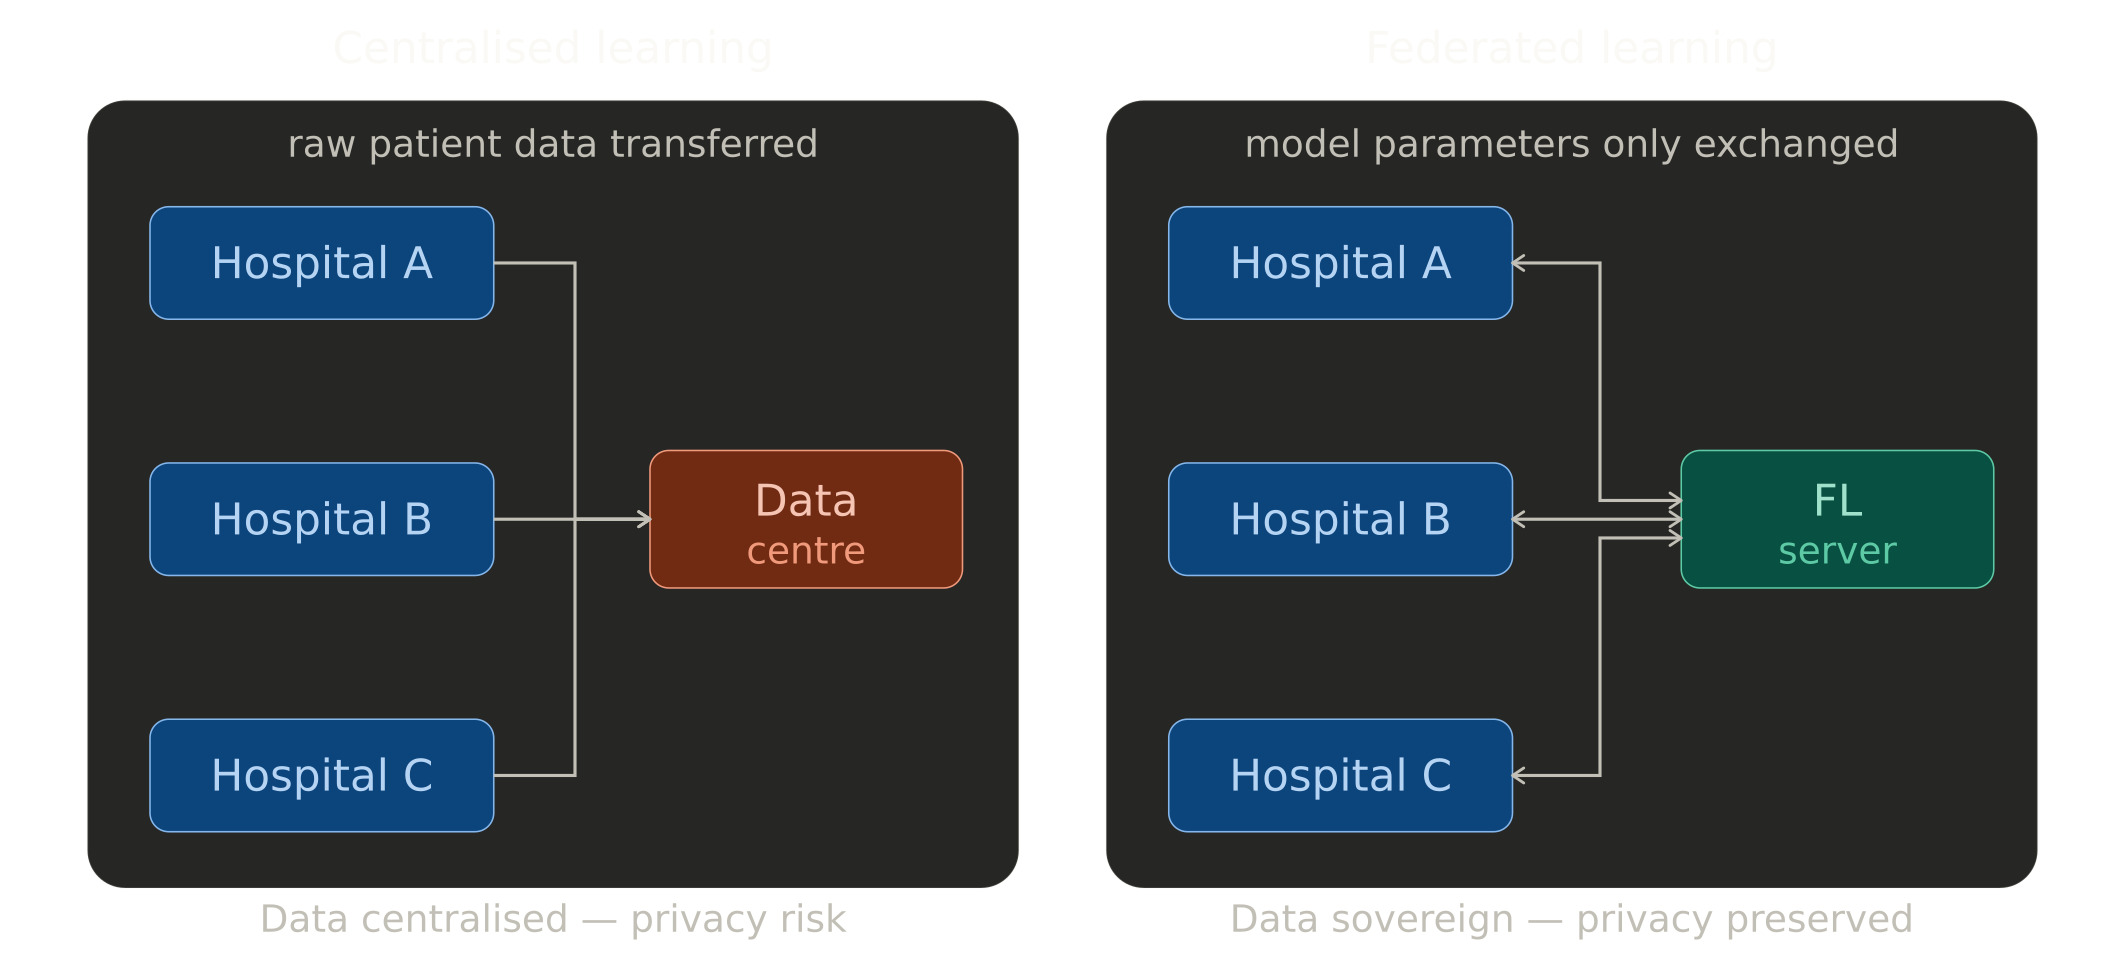
\includegraphics[width=\textwidth]{figures/fig2_1_centralised_vs_federated.jpg}
    \caption{Centralised versus federated learning in a multi-hospital
      breast MRI scenario. Left: raw patient data must be transferred
      to a single data centre, raising GDPR and data-sovereignty
      concerns \cite{gdpr2016regulation,hipaa1996health}. Right: only
      model parameters are exchanged with the coordination server;
      raw data remain at each institution \cite{mcmahan2017communication}.}
    \label{fig:centralised-vs-fl}
\end{figure}


\subsection{Distributed Learning Paradigms}
\label{sec:distributed-paradigms}

The limitations of centralised learning have motivated a spectrum of
distributed training approaches that differ in where data reside, how
computation is partitioned, and the degree of trust placed in the
coordinating infrastructure.
Understanding where federated learning sits within this spectrum
clarifies both its distinctive properties and the assumptions it makes.

\paragraph{Classical data-parallel distributed training.}
The most straightforward departure from single-machine training is
data-parallel processing in a parameter-server architecture
\cite{dean2012large}.
A central server maintains the canonical copy of model parameters;
a pool of worker machines each receive a disjoint shard of a centrally
stored dataset, compute gradients over that shard, and return the
gradients to the server for synchronous or asynchronous aggregation.
This architecture scales computation across many machines and has
become standard practice in industry for training large-scale models.
Crucially, however, the data themselves remain co-located in a shared
data centre under the exclusive control of a single operator.
Data-parallel distributed training therefore does not address the
privacy, sovereignty, or data-transfer cost concerns identified in the
previous section; it is an engineering technique for accelerating
computation over a centralised dataset, not a solution to the
multi-institutional data-governance problem.

\paragraph{Federated learning as a privacy-aware cross-silo paradigm.}
Federated learning introduces a qualitatively different constraint:
the training data are not co-located and, by design or by legal
requirement, cannot be moved to a central facility.
Each data silo -- referred to in the FL literature as a
\emph{client} -- retains its data locally and participates in the
training process by computing model updates on its own private dataset
and transmitting only those updates, never the raw data, to a
coordinating server \cite{mcmahan2017communication}.
The server aggregates parameter updates from participating clients and
broadcasts an improved global model for the next training round.
Raw patient records never traverse the network, and the communication
channel carries only floating-point model weights whose privacy
properties can be further reinforced with cryptographic or
noise-injection techniques (discussed in
Section~\ref{sec:privacy-security}).

FL is commonly classified along two orthogonal axes that determine the
applicable algorithms and privacy assumptions.
The first axis distinguishes \emph{horizontal} from \emph{vertical}
federation.
In \emph{horizontal} FL, all clients share the same feature space -- all
institutions acquire the same imaging modality and predict the same
outcome -- but hold non-overlapping patient populations.
This is the setting relevant to the present thesis: each of the three
simulated hospital clients holds a distinct cohort of breast MRI
patients with the same four molecular subtype labels.
In \emph{vertical} FL, clients hold overlapping patient identifiers
but complementary feature spaces -- for example, one institution holds
MRI images and another holds genomic profiles for the same patients.
Vertical federation requires patient-identifier alignment across sites,
which introduces additional privacy challenges and is a more complex
engineering problem \cite{yang2019federated,kairouz2021advances}.

The second axis distinguishes \emph{cross-device} from
\emph{cross-silo} federation.
Cross-device FL involves a very large number of lightweight,
intermittently available clients -- potentially millions of smartphones
or Internet-of-Things sensors -- communicating over unreliable
low-bandwidth links with highly heterogeneous hardware capabilities.
Cross-silo FL, by contrast, involves a small to moderate number of
institutional clients -- a consortium of hospitals or research
centres -- that are persistently available, possess substantial compute
resources, and are typically bound by formal data-sharing agreements
even if raw data transfer is prohibited.
The breast MRI classification scenario studied in this work corresponds
to \emph{cross-silo horizontal} FL: three simulated hospital clients,
each holding a non-IID partition of the 737-patient DCE-MRI dataset,
trained using the Flower framework with PyTorch as the local compute
backend.
Table~\ref{tab:fl-taxonomy} summarises the key distinctions between
the main FL paradigms.

\begin{table}[htbp]
  \centering
  \caption{Taxonomy of federated learning paradigms along two
    classification axes. This thesis operates in the cross-silo,
    horizontal quadrant.}
  \label{tab:fl-taxonomy}
  \renewcommand{\arraystretch}{1.3}
  \begin{tabular}{lll}
    \hline
    \textbf{Axis} & \textbf{Category} & \textbf{Characteristics} \\
    \hline
    \multirow{2}{*}{Data partition}
      & Horizontal FL & Same features, different patients \\
      & Vertical FL   & Same patients, complementary features \\
    \hline
    \multirow{2}{*}{Client scale}
      & Cross-device FL & Millions of clients; intermittent, heterogeneous \\
      & Cross-silo FL   & Tens of clients; persistent, institutional \\
    \hline
  \end{tabular}
\end{table}

\begin{figure}[htbp]
    \centering
    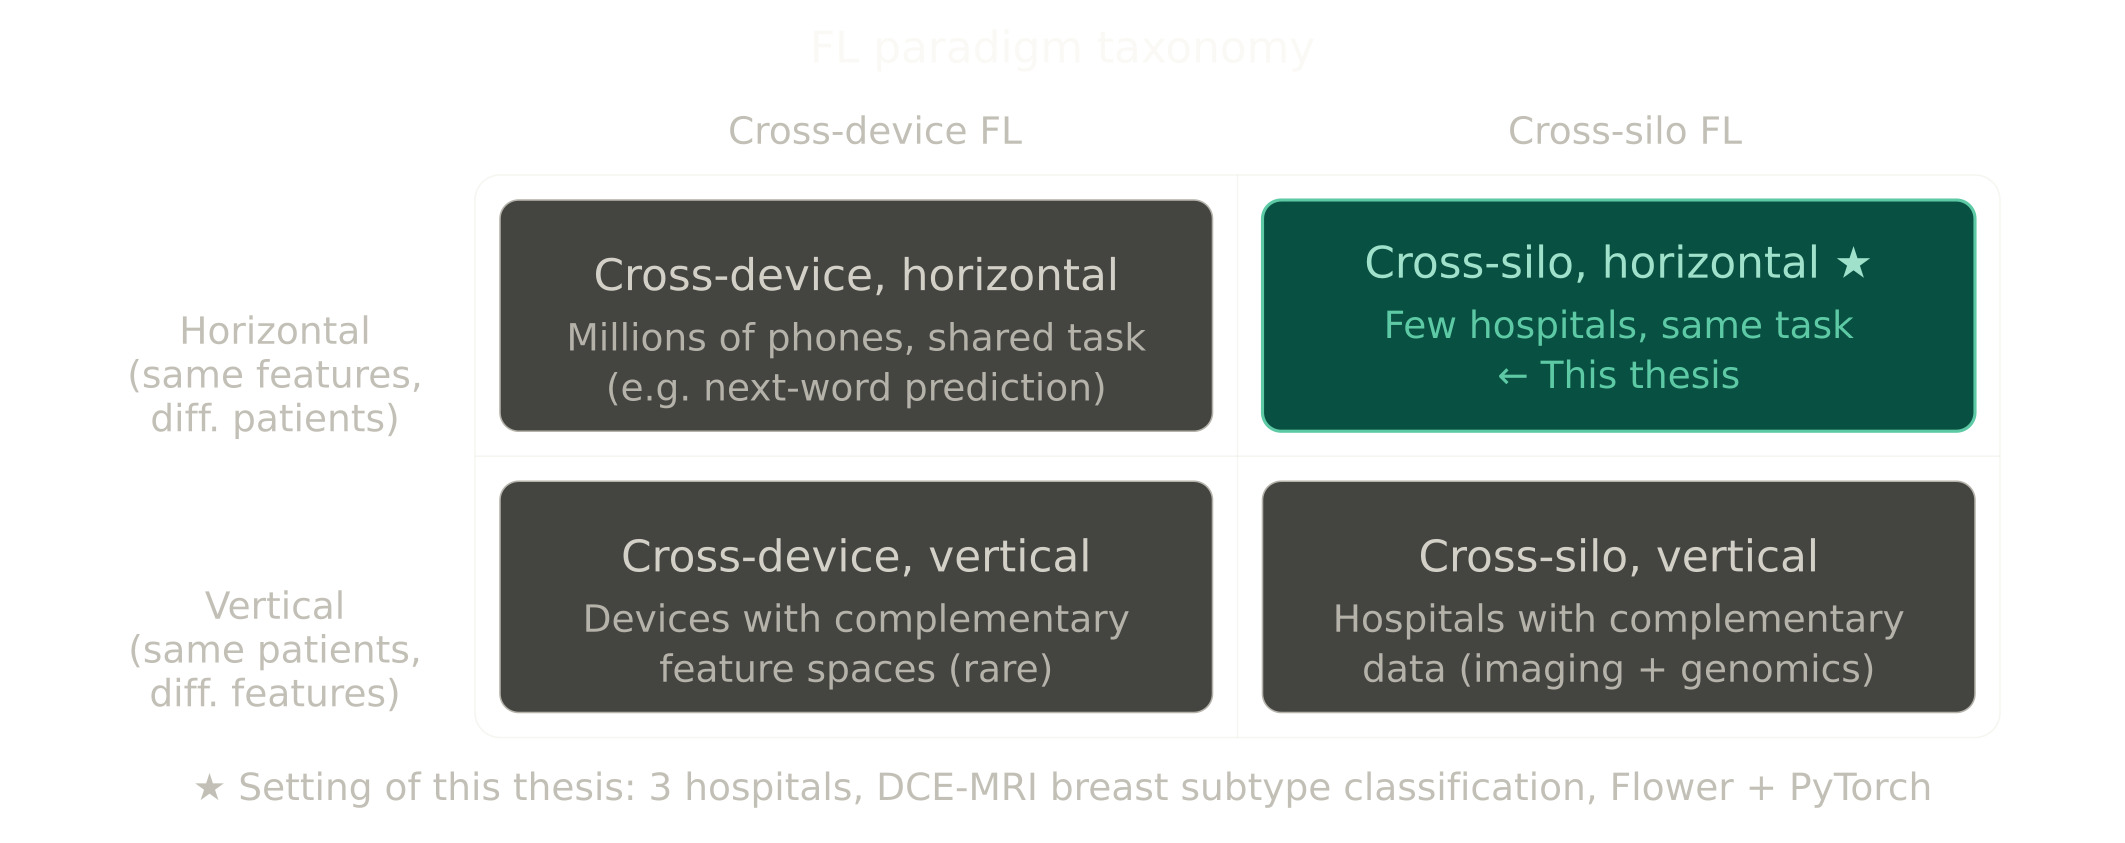
\includegraphics[width=0.8\textwidth]{figures/fig2_2_fl_taxonomy.jpg}
    \caption{Taxonomy of federated learning paradigms. The highlighted
      quadrant -- cross-silo, horizontal FL -- corresponds to the
      setting adopted in this thesis \cite{yang2019federated,kairouz2021advances}.}
    \label{fig:fl-taxonomy}
\end{figure}


\subsection{Definition and Origins of Federated Learning}
\label{sec:fl-definition}

Federated learning was formally introduced by McMahan \emph{et al.}\
in 2017 in the context of training a next-word-prediction language
model on data distributed across millions of mobile devices
\cite{mcmahan2017communication}.
The authors identified a class of learning problems characterised by
three properties: the training data are generated and stored on devices
that are not under the operator's direct control; those data contain
sensitive user information that makes centralised aggregation
undesirable; and the dataset is massively distributed, with each
device holding a relatively small and non-identically distributed
portion of the total information.
The proposed solution -- \emph{Federated Averaging} (FedAvg) -- has since
become the canonical baseline algorithm for the field and is described
in detail in Section~\ref{sec:fedavg}.

Formally, the federated learning optimisation problem is stated as
follows.
Let $K$ denote the number of participating clients, let
$\mathcal{D}_k$ denote the private local dataset of client $k$,
with $n_k = |\mathcal{D}_k|$ the number of local samples and
$n = \sum_{k=1}^{K} n_k$ the total sample count across all clients.
The goal is to find model parameters $\mathbf{w}^{\ast}$ that minimise
the globally weighted empirical risk:

\begin{equation}
  \mathbf{w}^{\ast}
  \;=\;
  \arg\min_{\mathbf{w} \in \mathbb{R}^d}
  \sum_{k=1}^{K} \frac{n_k}{n}\, F_k(\mathbf{w}),
  \label{eq:fl-objective}
\end{equation}

where the local objective $F_k$ of client $k$ is the empirical risk
over its private data:

\begin{equation}
  F_k(\mathbf{w})
  \;=\;
  \frac{1}{n_k}
  \sum_{(\mathbf{x},\, y)\,\in\,\mathcal{D}_k}
  \ell\bigl(f(\mathbf{x};\mathbf{w}),\; y\bigr),
  \label{eq:local-risk}
\end{equation}

with $f(\cdot\,;\mathbf{w})$ the model function parameterised by
$\mathbf{w}$, and $\ell$ the per-sample loss function (e.g.\
cross-entropy for multi-class classification).
The key observation is that the objective in
\eqref{eq:fl-objective} is \emph{mathematically equivalent} to
standard empirical risk minimisation over the pooled dataset
$\bigcup_k \mathcal{D}_k$, yet it can be minimised
\emph{without ever pooling the data} \cite{kairouz2021advances}.

Training proceeds in discrete \emph{communication rounds}.
At round $t$, the server selects a subset of clients
$\mathcal{S}^{(t)} \subseteq \{1,\ldots,K\}$ and broadcasts the
current global parameters $\mathbf{w}^{(t)}$.
Each selected client $k$ initialises its local model with
$\mathbf{w}^{(t)}$ and performs $E$ steps of mini-batch stochastic
gradient descent on $\mathcal{D}_k$, obtaining a locally updated
parameter vector $\mathbf{w}_k^{(t+1)}$.
The server then aggregates the client updates into a new global
model using a weighted average:

\begin{equation}
  \mathbf{w}^{(t+1)}
  \;=\;
  \sum_{k\,\in\,\mathcal{S}^{(t)}}
  \frac{n_k}{\displaystyle\sum_{j\,\in\,\mathcal{S}^{(t)}} n_j}\;
  \mathbf{w}_k^{(t+1)}.
  \label{eq:fedavg-aggregation}
\end{equation}

Equation~\eqref{eq:fedavg-aggregation} is the aggregation step of
FedAvg; the local training step and its interaction with data
heterogeneity are analysed in detail in Section~\ref{sec:aggregation}.

The transition from the original mobile cross-device setting to
cross-silo healthcare applications was both rapid and well-motivated.
Pioneering empirical work by Sheller \emph{et al.}\ demonstrated
that a FL model trained across multiple institutions, without any
data sharing, could achieve performance competitive with a centrally
trained baseline on a brain tumour segmentation task -- a result
attributable in part to the regularising effect of training on
heterogeneous clinical distributions \cite{sheller2020federated}.
Subsequent comprehensive surveys have catalogued FL applications
spanning radiology, pathology, genomics, and electronic health records
\cite{rieke2020future,nguyen2022federated,kaissis2020secure},
establishing federated learning as the dominant collaborative learning
paradigm endorsed by the medical AI research community when privacy
constraints prohibit raw data sharing.

\begin{figure}[htbp]
    \centering
    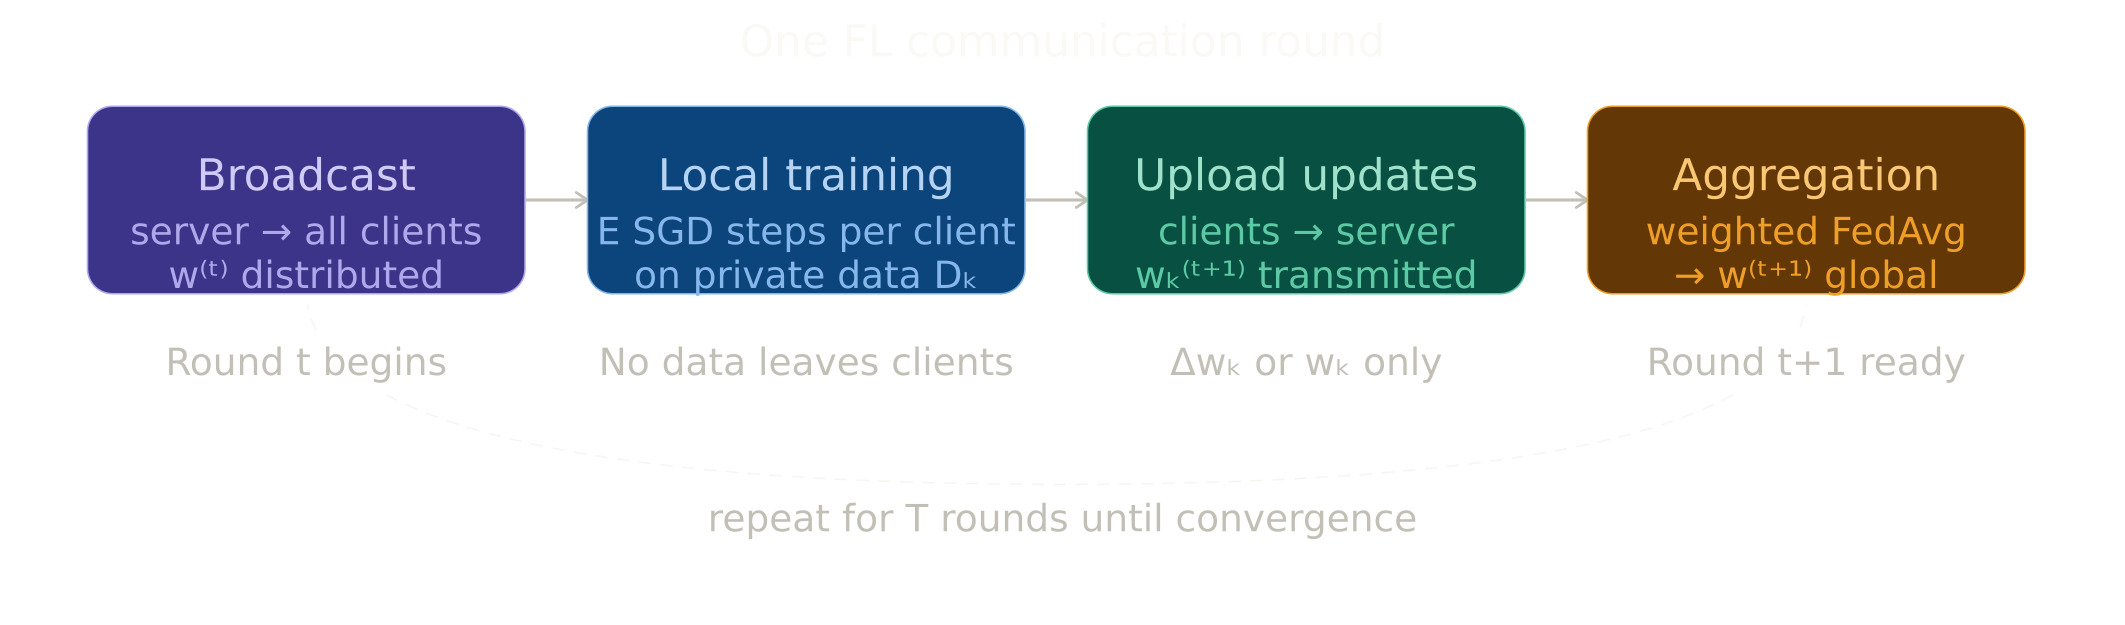
\includegraphics[width=\textwidth]{figures/fig2_3_one_fl_round.jpg}
    \caption{The four phases of one federated learning communication
      round (equation~\eqref{eq:fedavg-aggregation}). The server
      broadcasts $\mathbf{w}^{(t)}$, each client performs $E$ local
      SGD steps on $\mathcal{D}_k$, the resulting
      $\mathbf{w}_k^{(t+1)}$ are uploaded, and the server computes
      the weighted aggregate $\mathbf{w}^{(t+1)}$
      \cite{mcmahan2017communication,kairouz2021advances}.}
    \label{fig:fl-round}
\end{figure}


% ============================================================
\section{Federated Learning Architecture}
\label{sec:fl-architecture}
% ============================================================

The practical realisation of the federated optimisation objective
defined in Section~\ref{sec:fl-definition} requires a concrete system
architecture that coordinates communication between geographically
distributed participants, manages model state across training rounds,
and enforces the data-locality constraint that distinguishes federated
from centralised learning.
This section describes the canonical two-tier client--server
architecture that underlies most deployed and experimental FL systems,
including the Flower-based setup employed in this thesis.

\subsection{Client-Server Paradigm}
\label{sec:client-server}

The canonical FL architecture is organised as a two-tier hierarchy
consisting of a central coordination server and a set of $K$ clients,
each in possession of a private local dataset $\mathcal{D}_k$ that
remains on-site throughout the entire training process
\cite{mcmahan2017communication}.
The server is the orchestrating entity: it maintains the authoritative
copy of the global model, schedules training rounds, selects
participating clients, aggregates locally computed updates, and
broadcasts the updated global model.
Clients are the computational entities: each executes local
optimisation on its own data and returns parameter updates to the
server without exposing raw records.

This division of responsibility reflects both the privacy requirement
and the typical infrastructure of cross-silo healthcare deployments.
The server may be hosted by a neutral third party -- a research
consortium, a cloud provider operating under a data-processing
agreement, or one of the participating hospitals designated as
coordinator -- provided that the server never receives raw patient data.
Clients in a cross-silo setting are typically individual hospital sites
or research centres, each equipped with sufficient GPU compute to
execute local training on their imaging datasets
\cite{rieke2020future,kairouz2021advances}.

An important architectural distinction concerns the degree of client
selection per round.
In large-scale cross-device FL, only a small fraction of available
clients participate in each round due to device availability and
bandwidth constraints.
In cross-silo deployments of the kind considered in this thesis, where
the total number of clients is small (three simulated hospital nodes),
all clients participate in every round, simplifying convergence
analysis and eliminating the client-dropout variability that
complicates cross-device FL \cite{kairouz2021advances}.

\subsection{Local Training at Client Institutions}
\label{sec:local-training}

At the commencement of each communication round $t$, every selected
client $k \in \mathcal{S}^{(t)}$ receives the current global parameter
vector $\mathbf{w}^{(t)}$ from the server and initialises its local
model with this shared starting point.
The client then performs a fixed number $E$ of local optimisation
steps using mini-batch stochastic gradient descent (SGD) over its
private dataset $\mathcal{D}_k$, minimising the local empirical risk
$F_k(\mathbf{w})$ defined in equation~\eqref{eq:local-risk}.

The choice of $E$ governs the trade-off between communication
efficiency and optimisation quality.
A single local step ($E = 1$) reduces to synchronous distributed SGD
and requires a communication round after every gradient computation,
incurring high bandwidth costs.
Multiple local steps ($E > 1$) amortise the communication overhead
across more computation but introduce \emph{client drift}: because
each client optimises its local objective rather than the global one,
the local model moves away from the global optimum at a rate that
depends on the statistical heterogeneity of the local data distribution
\cite{kairouz2021advances}.
In the non-IID setting characteristic of multi-hospital deployments --
where patient demographics, scanner protocols, and subtype prevalence
differ across sites -- client drift is a primary source of convergence
degradation and motivates the regularisation techniques discussed in
Section~\ref{sec:aggregation}.

In the breast MRI molecular subtype classification scenario of this
thesis, each client applies the same ResNet-based backbone architecture
initialised from the global weights, performing local updates using a
cosine learning rate schedule with MixUp augmentation to mitigate the
class imbalance arising from the non-IID partition of the 737-patient
dataset across three hospital nodes.
Progressive unfreezing of backbone layers during local training is
employed to preserve low-level feature representations learned from the
global model while adapting higher-level features to site-specific data
characteristics.

\subsection{Global Model Aggregation on the Server}
\label{sec:global-aggregation}

Upon completion of local training, each participating client $k$
transmits its updated local parameter vector $\mathbf{w}_k^{(t+1)}$
to the central server.
The server's aggregation function combines these client updates into a
new global model that, under the weighted averaging scheme of FedAvg,
corresponds to the sample-size-weighted mean of local parameters as
given in equation~\eqref{eq:fedavg-aggregation}.
The resulting global model $\mathbf{w}^{(t+1)}$ integrates knowledge
from all participating clients without requiring any client to share
its underlying data.

The correctness of weighted averaging as an aggregation operator rests
on the assumption that local models are trained from the same
initialisation and that the global objective is the weighted sum of
local objectives with weights proportional to dataset size
\cite{mcmahan2017communication}.
Under these conditions, averaging in parameter space approximates a
single gradient step on the global objective.
When the assumption of identical data distributions across clients is
violated -- the non-IID case -- this approximation degrades, and the
aggregated model may converge to a point that is suboptimal for all
clients simultaneously.
Alternative aggregation strategies that address this degradation are
surveyed in Section~\ref{sec:aggregation}.

A practical consideration in cross-silo medical imaging deployments is
the size of the parameter vectors being transmitted.
A ResNet-50 backbone comprises approximately 25 million floating-point
parameters; transmitting full parameter vectors from three hospital
clients per round is feasible within the bandwidth constraints of
institutional networks, in contrast to the gradient-compression
requirements of cross-device deployments involving thousands of
participants \cite{kairouz2021advances,rieke2020future}.

\subsection{Communication Rounds and Convergence}
\label{sec:comm-rounds}

Training in federated learning is structured as a sequence of discrete
communication rounds rather than the continuous gradient flow of
centralised training.
Each round consists of four steps: the server broadcasts the current
global model to selected clients; clients perform local optimisation;
clients transmit updated parameters to the server; and the server
aggregates the updates and prepares the next global model.
This round structure introduces a fundamental coupling between the
number of communication rounds $T$, the number of local steps $E$ per
round, and the total computational budget available to each client.

Convergence analysis for FedAvg under non-IID data distributions
demonstrates that the algorithm converges at a rate that degrades as
the degree of data heterogeneity -- measured by the gradient divergence
$\|\nabla F_k(\mathbf{w}) - \nabla F(\mathbf{w})\|$ across clients --
increases \cite{kairouz2021advances}.
Intuitively, when local data distributions differ substantially, local
gradient directions point towards different local optima, and their
average after multiple local steps is a poor approximation to the
global gradient.
The practical consequence is that non-IID FL systems may require
significantly more communication rounds to achieve a given target
accuracy than an equivalent centralised system trained on the pooled
dataset.

In healthcare FL deployments, the number of communication rounds is
also constrained by institutional factors beyond pure optimisation
considerations: each round involves synchronisation across hospital
sites that may operate on different schedules, under different
computational loads, and subject to network availability constraints
that do not arise in a single data centre.
For the three-hospital simulation in this thesis, all clients are
available synchronously, so round scheduling reduces to a hyperparameter
choice; the interaction between round count, local epochs, and
convergence on the non-IID breast MRI partition is reported in
Chapter~3.


% ============================================================
%  STUB SECTIONS 2.4 -- 2.10
%  Labels only -- prose to be filled in progressively.
%  Do NOT remove these stubs until the section is fully written;
%  they resolve all forward \ref{} calls from sections above.
% ============================================================

\section{Aggregation Strategies}
\label{sec:aggregation}
% TODO: Write section 2.4 (FedAvg variants, FedProx, FedNova, SCAFFOLD, personalised FL)

\subsection{Federated Averaging}
\label{sec:fedavg}
% TODO: Write 2.4.1 -- detailed FedAvg walkthrough (referenced from sec:fl-definition)

\section{Communication Protocols and Optimisation}
\label{sec:communication}
% TODO: Write section 2.5 (gradient compression, quantisation, asynchronous FL)

\section{Privacy and Security in Federated Learning}
\label{sec:privacy-security}
% TODO: Write section 2.6 (threat models, DP, secure aggregation, HE)

\section{Convergence and Stability Challenges}
\label{sec:convergence}
% TODO: Write section 2.7 (non-IID impact, system heterogeneity, stabilisation)

\section{Federated Learning Frameworks}
\label{sec:frameworks}
% TODO: Write section 2.8 (Flower, FedML, Substra, PySyft, comparison)

\section{Related Work}
\label{sec:related-work}
% TODO: Write section 2.9 (FL in EEG, medical imaging, oncology; positioning)

\section{Conclusion}
\label{sec:ch2-conclusion}
% TODO: Write section 2.10

% \chapter{Chapter 3 -- Proposed Architecture and Methodology}

\section{Introduction}

\section{Overall System Architecture}

\subsection{General Design of the Federated System}
\subsection{Federation Topology (Number of Clients, Server Role)}
\subsection{Multi-Modality Integration Strategy}

\section{Case Study 1 — EEG Signals for Epilepsy Detection}

\subsection{Dataset Description and Sources}
\subsection{EEG Signal Preprocessing}

\subsubsection{Filtering and Artifact Removal}
\subsubsection{Segmentation and Epoching}


\subsection{Feature Extraction}

\subsubsection{Time-Domain Features}
\subsubsection{Frequency-Domain Features}


\subsection{Local Model Architecture for EEG Classification}

\section{Case Study 2 — Medical Imaging for Cancer Sub-Type Classification}

\subsection{Dataset Description and Sources}
\subsection{Image Preprocessing}

\subsubsection{Normalization and Resizing}
\subsubsection{Data Augmentation}


\subsection{Local Model Architecture for Image Classification}

\subsubsection{CNN-Based Architecture}
\subsubsection{Transfer Learning Strategy}



\section{Proposed Aggregation Strategy Optimizations}

\subsection{Baseline: FedAvg}
\subsection{Proposed Variants and Modifications}
\subsection{Adaptive Weighting of Client Contributions}
\subsection{Handling Non-IID Data Across Institutions}

\section{Proposed Communication Scheme Optimizations}

\subsection{Gradient Compression Strategy}
\subsection{Communication Round Scheduling}
\subsection{Bandwidth-Efficient Update Transmission}

\section{Privacy Preservation Mechanisms}

\subsection{Applied Differential Privacy Configuration}
\subsection{Secure Aggregation Protocol}

\section{Evaluation Protocol}

\subsection{Federated vs. Centralized Baseline Comparison}
\subsection{Cross-Validation Strategy}
\subsection{Performance Metrics per Task}
\subsection{Convergence Monitoring Metrics}
\section{Conclusion}


% % ============================================================
%  CHAPTER 4 — IMPLEMENTATION AND RESULTS
%
%  ALL CONFIRMED VALUES:
%  4-class macro F1     = 0.3424  (bootstrap mean 0.3411)
%  95% CI               = [0.301, 0.382]
%  Balanced accuracy    = 0.3688
%  AUC-ROC (macro OvR)  = 0.6009
%  Brier score          = 0.6814
%  Per-class F1: LumA=0.63, LumB=0.22, HER2=0.20, TN=0.33
%  Fold F1: 0.3231, 0.3401, 0.3682, 0.3699, ~0.3107
%  FL: R=50, E=5, K=3, binary, Dir(0.5)
%  TODO markers: binary results, FL results, confusion matrix,
%  ROC curves, SCAFFOLD results
% ============================================================

\chapter{Implementation and Results}
\label{chap:results}

% ============================================================
\section{Introduction}
\label{sec:ch4-intro}
% ============================================================

This chapter presents the implementation details and experimental
results of the two studies described in Chapter~3.
Section~\ref{sec:hardware} documents the hardware and software
environment.
Section~\ref{sec:fed-system-setup} describes the configuration
of the federated simulation.
Section~\ref{sec:centralised-results} reports the five-fold
cross-validated performance of the centralised ConvNeXt-Nano
plus Gated Attention MIL pipeline on the four-class molecular
subtype task, establishing the performance ceiling against which
the federated system is evaluated.
Section~\ref{sec:fl-results} presents the federated learning
results under FedAvg and SCAFFOLD aggregation on the binary
Luminal versus Non-Luminal reformulation.
Section~\ref{sec:convergence-results} analyses convergence
behaviour across communication rounds.
Section~\ref{sec:classification-performance} provides detailed
per-class evaluation including confusion matrices and ROC curves.
Section~\ref{sec:sota-comparison} positions the results within
the related literature.
Section~\ref{sec:ch4-conclusion} concludes the chapter.


% ============================================================
\section{Hardware and Software Environment}
\label{sec:hardware}
% ============================================================

\subsection{Hardware Specifications}
\label{sec:hardware-specs}

All experiments were conducted on a single workstation whose
specifications are summarised in Table~\ref{tab:hardware}.
The GPU memory constraint of 6~GB is the primary driver of
several design decisions described in Chapter~3, including the
use of gradient checkpointing, the physical batch size of~2
with gradient accumulation, and the two-chunk forward pass
strategy in the MIL head.

\begin{table}[htbp]
  \centering
  \caption{Hardware specifications of the experimental workstation.}
  \label{tab:hardware}
  \renewcommand{\arraystretch}{1.3}
  \begin{tabular}{ll}
    \toprule
    \textbf{Component} & \textbf{Specification} \\
    \midrule
    GPU   & NVIDIA GeForce GTX 1660 Ti, 6 GB GDDR6 \\
    CPU   & Intel Core i5-13400 (10 cores, 4.6 GHz boost) \\
    RAM   & 16 GB DDR4 \\
    Storage & NVMe SSD \\
    OS    & Windows 11 with WSL2 / PowerShell \\
    \bottomrule
  \end{tabular}
\end{table}

\subsection{Software Environment}
\label{sec:software-env}

The software stack is listed in Table~\ref{tab:software}.
PyTorch~2.1.2 with CUDA~11.8 provides the deep learning
backend.
The \texttt{timm} library supplies the pretrained
ConvNeXt-Nano weights and model construction utilities.
Flower provides the federated learning simulation framework.
SimpleITK handles MRI volume loading and spatial resampling.
PyRadiomics performs the hand-crafted feature extraction
described in Section~\ref{sec:radiomics}.

\begin{table}[htbp]
  \centering
  \caption{Software stack used throughout all experiments.}
  \label{tab:software}
  \renewcommand{\arraystretch}{1.3}
  \begin{tabular}{lll}
    \toprule
    \textbf{Library} & \textbf{Version} & \textbf{Role} \\
    \midrule
    PyTorch     & 2.1.2+cu118 & Deep learning backend \\
    timm        & 0.9.16      & Pretrained backbone \\
    Flower      & 1.x         & FL simulation \\
    MONAI       & 1.3.0       & Medical imaging utilities \\
    SimpleITK   & 2.x         & Volume loading \\
    PyRadiomics & 3.x         & Feature extraction \\
    scikit-learn & 1.x        & Cross-validation, metrics \\
    NumPy       & $<$2.0      & Numerical operations \\
    \bottomrule
  \end{tabular}
\end{table}

\subsection{Development Tools}
\label{sec:dev-tools}

Training runs were launched via PowerShell using the command:
\begin{verbatim}
python -u main.py --arch convnext_mil --stage all --fold N
    | Tee-Object -FilePath logs/foldN.log
\end{verbatim}
which simultaneously displays and persists training metrics.
The environment variable \texttt{HF\_HUB\_OFFLINE=1} was set
after the first model download to prevent unintended network
requests.
All random seeds are fixed via \texttt{seed=42} in the
\texttt{StratifiedGroupKFold} split and via per-seed
initialisation in the Stage~3 cRT loop to ensure
reproducibility.


% ============================================================
\section{Federated System Configuration}
\label{sec:fed-system-setup}
% ============================================================

\subsection{Simulation of Federated Clients}
\label{sec:client-simulation}

The federated experiment is conducted in Flower's simulation
mode, which executes all three client processes sequentially
on the single available GPU rather than in parallel across
network nodes.
This approach is standard in FL research when the goal is
to evaluate algorithmic properties rather than network
infrastructure \cite{beutel2022flower}.
Sequential execution introduces no algorithmic difference
relative to a true parallel deployment: each client receives
an identical copy of the global model, trains independently
on its local partition, and returns its parameter vector
before the next client begins.

\subsection{Data Partitioning}
\label{sec:data-partitioning}

The 737 binary-labelled patients (557 Luminal, 180
Non-Luminal) are partitioned across three clients using the
Dirichlet strategy with $\alpha = 0.5$ as described in
Section~\ref{sec:noniid-partition}.
Table~\ref{tab:client-partition} reports the resulting
per-client sample counts and local imbalance ratios for the
seed used in the primary experiment.

\begin{table}[htbp]
  \centering
  \caption{Binary data partition across three simulated
    hospital clients under Dirichlet $\alpha=0.5$.}
  \label{tab:client-partition}
  \renewcommand{\arraystretch}{1.3}
  \begin{tabular}{lcccc}
    \toprule
    \textbf{Client} & \textbf{Luminal}
      & \textbf{Non-Luminal} & \textbf{Total}
      & \textbf{Local ratio} \\
    \midrule
    Hospital 1 & 300 & 38  & 338 & 7.9:1 \\
    Hospital 2 & 180 & 108 & 288 & 1.7:1 \\
    Hospital 3 & 77  & 34  & 111 & 2.3:1 \\
    \midrule
    \textbf{Total} & \textbf{557} & \textbf{180}
      & \textbf{737} & \textbf{3.1:1} \\
    \bottomrule
  \end{tabular}
\end{table}

\subsection{Communication Round Configuration}
\label{sec:round-config}

The federated training runs for $R = 50$ communication
rounds, which is sufficient to observe convergence in
cross-silo settings with small cohorts
\cite{sheller2020federated}.
Each selected client performs $E = 5$ local training epochs
per round before uploading its parameters.
All three clients participate in every round ($C = 1.0$,
full participation), consistent with the persistent
availability assumption of cross-silo federation.
The total local compute per round is therefore
$K \times E = 15$ client-epochs, and the aggregate local
compute over the full experiment is $R \times K \times E
= 750$ client-epochs.


% ============================================================
\section{Centralised Baseline Results}
\label{sec:centralised-results}
% ============================================================

\subsection{Five-Fold Cross-Validation Performance}
\label{sec:fivefold-results}

Table~\ref{tab:fold-results} presents the per-fold and
aggregate cRT macro F1 scores for the four-class
centralised experiment.
The five-fold ensemble achieves a macro F1 of $0.342$
(bootstrap 95\% CI: $[0.301,\; 0.382]$), a balanced
accuracy of $0.369$, and a macro one-versus-rest AUC-ROC
of $0.601$.
These metrics constitute the performance ceiling of the
system and the primary reference against which the
federated experiment is evaluated.

\begin{table}[htbp]
  \centering
  \caption{Per-fold cRT macro F1 scores and ensemble
    aggregate metrics for the four-class centralised
    experiment. CI~=~confidence interval computed by
    bootstrap resampling ($n=1000$).}
  \label{tab:fold-results}
  \renewcommand{\arraystretch}{1.3}
  \begin{tabular}{lc}
    \toprule
    \textbf{Fold / Metric} & \textbf{Value} \\
    \midrule
    Fold 0 (cRT) & 0.3231 \\
    Fold 1 (cRT) & 0.3401 \\
    Fold 2 (cRT) & 0.3682 \\
    Fold 3 (cRT) & 0.3699 \\
    Fold 4 (cRT) & $\approx 0.31$ \\
    \midrule
    \textbf{Ensemble macro F1} & \textbf{0.3424} \\
    Bootstrap mean F1          & 0.3411 \\
    95\% CI                    & [0.301,\ 0.382] \\
    Balanced accuracy          & 0.3688 \\
    AUC-ROC (macro OvR)        & 0.6009 \\
    Brier score                & 0.6814 \\
    \bottomrule
  \end{tabular}
\end{table}

\subsection{Per-Class Analysis}
\label{sec:perclass-results}

Table~\ref{tab:perclass-results} disaggregates the ensemble
performance by molecular subtype.
The results reveal a clear stratification that reflects the
class frequency distribution of the dataset.

\begin{table}[htbp]
  \centering
  \caption{Per-class precision, recall, and F1-score for the
    five-fold ensemble on the four-class task.
    Support column shows the total number of patients per
    class across all five validation folds.}
  \label{tab:perclass-results}
  \renewcommand{\arraystretch}{1.3}
  \begin{tabular}{lcccc}
    \toprule
    \textbf{Subtype} & \textbf{Precision}
      & \textbf{Recall} & \textbf{F1} & \textbf{Support} \\
    \midrule
    Luminal A       & 0.71 & 0.56 & 0.63 & 481 \\
    Luminal B       & 0.21 & 0.22 & 0.22 &  76 \\
    HER2-enriched   & 0.15 & 0.30 & 0.20 &  46 \\
    Triple Negative & 0.29 & 0.39 & 0.33 & 134 \\
    \midrule
    Macro average   & 0.34 & 0.37 & 0.34 & 737 \\
    Weighted average& 0.55 & 0.48 & 0.50 & 737 \\
    \bottomrule
  \end{tabular}
\end{table}

Luminal~A achieves the highest F1 of $0.63$, consistent
with its dominance of the training distribution at 65.3\%.
Triple-Negative achieves F1~$= 0.33$ despite representing
only 18.2\% of cases, suggesting that its imaging
phenotype is sufficiently distinctive for the backbone to
learn partial discrimination.
Luminal~B and HER2-enriched achieve the lowest F1 scores
of $0.22$ and $0.20$ respectively.
The HER2 result is particularly constrained: with only 46
total samples and approximately nine patients per validation
fold, a single misclassification shifts the per-class F1
by approximately 0.08 points, making the metric
statistically unstable at this sample size.
The precision of $0.15$ for HER2 indicates that the model
predicts this class frequently but correctly only in a
minority of cases, consistent with a strategy of generous
positive prediction to recover recall under LDAM.

\begin{figure}[htbp]
  \centering
  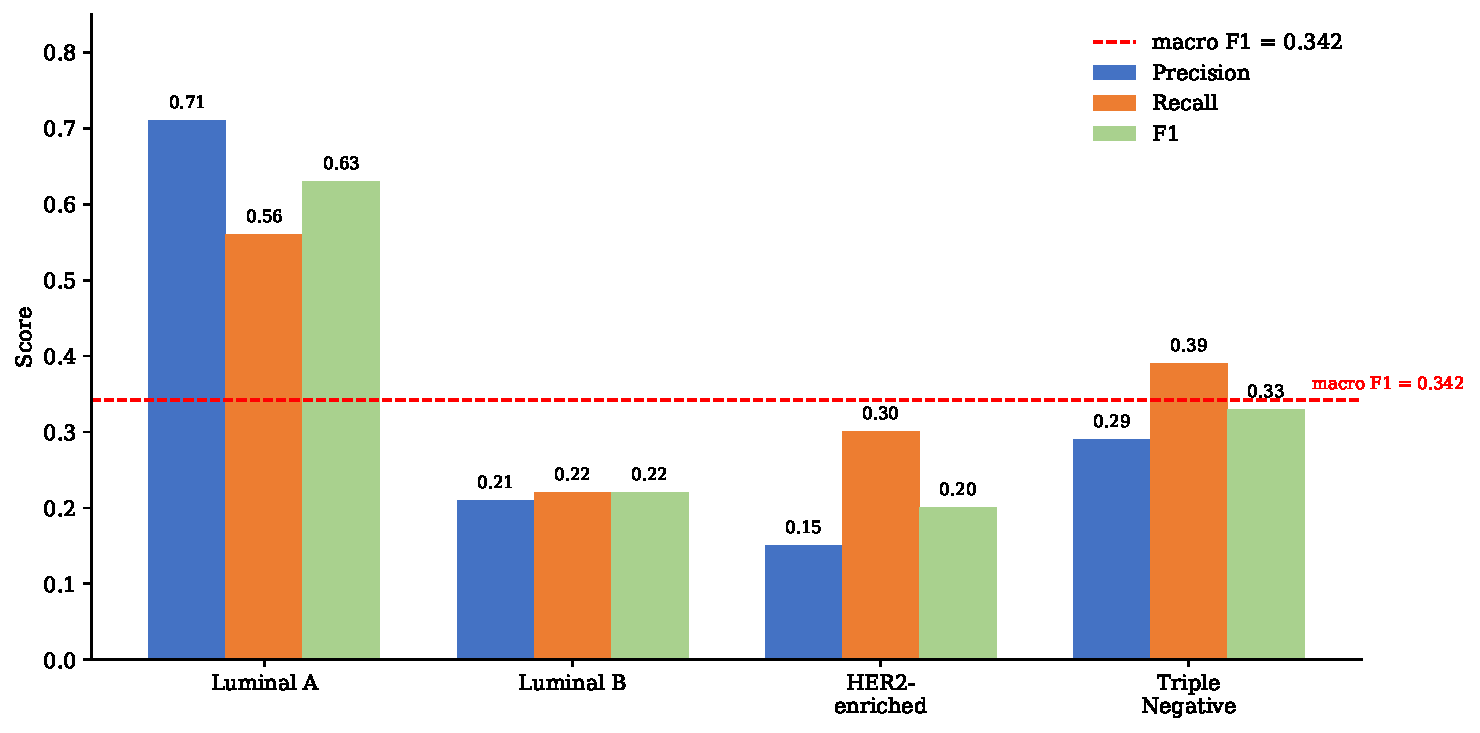
\includegraphics[width=0.92\linewidth]{figures/ch4_perclass_metrics.pdf}
  \caption{Per-class precision, recall, and F1-score for
    the five-fold ensemble on the four-class centralised
    task. The strong Luminal~A performance reflects its
    65.3\% majority status. HER2 achieves the lowest F1
    ($0.20$) due to the fundamental constraint of only
    46 training samples.}
  \label{fig:perclass-metrics}
\end{figure}

\begin{figure}[htbp]
  \centering
  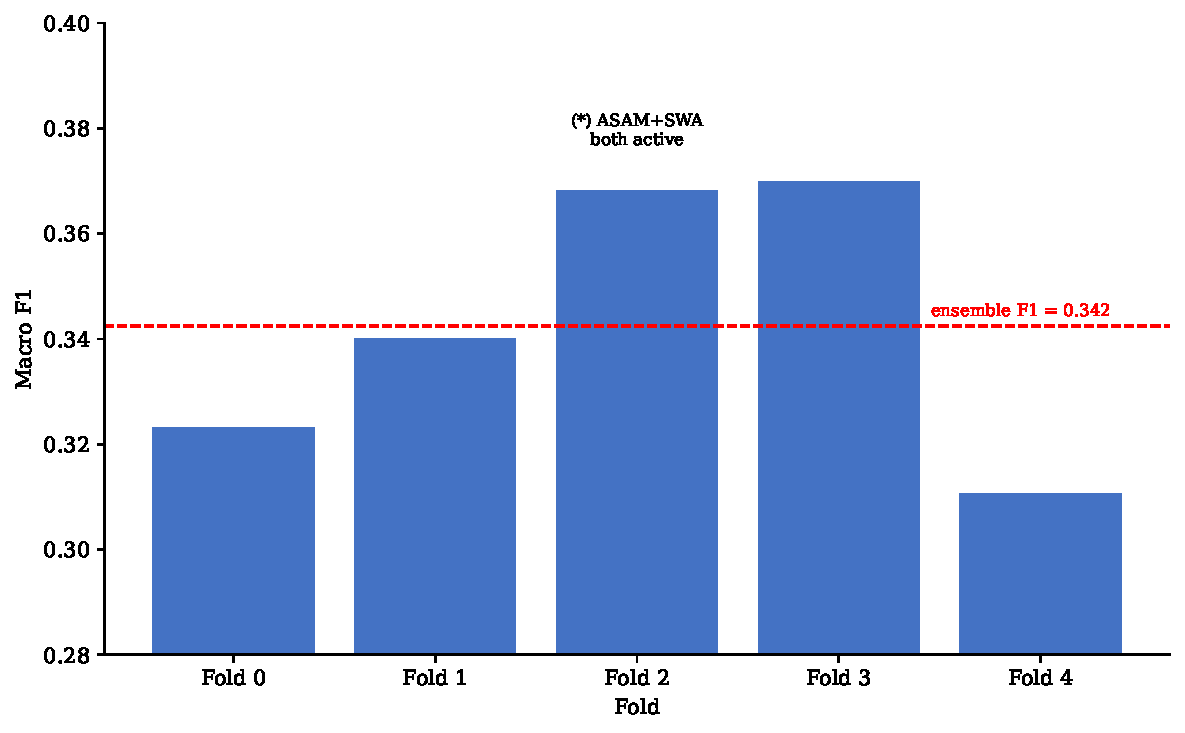
\includegraphics[width=0.80\linewidth]{figures/ch4_fold_f1.pdf}
  \caption{Per-fold cRT macro F1 scores across the five
    cross-validation folds. Folds~2 and~3 benefit from
    the first complete activations of ASAM (epoch~55)
    and SWA (epoch~65), breaking the convergence plateau
    observed in folds~0 and~1 where early training
    interruptions prevented full Stage~2 completion.}
  \label{fig:fold-f1}
\end{figure}

\subsection{Four-Class Performance Ceiling}
\label{sec:four-class-ceiling}

The ensemble macro F1 of $0.342$ (95\% CI: $[0.301,
0.382]$) represents the performance ceiling achievable
by a single-institution centralised system on this
dataset.
The HER2 F1 of $0.20$ reflects the fundamental constraint
of 46 training samples in the minority class: no
combination of loss reweighting, attention mechanisms,
or regularisation can substitute for sufficient training
data at this scale.
This ceiling motivates the binary reformulation
(Section~\ref{sec:binary-task}), which merges the two
rarest classes to produce a more tractable 3.1:1 imbalance
ratio, and the federated experiment, which simulates the
multi-institutional data pooling that would otherwise be
required to address this scarcity.
The macro AUC-ROC of $0.601$ confirms that the model
has learned meaningful discriminative information beyond
random chance ($0.50$), particularly for Luminal~A and
Triple-Negative subtypes where the class-specific AUCs
are substantially above the macro average.


% ============================================================
\section{Federated Learning Results}
\label{sec:fl-results}
% ============================================================

% TODO — fill when FL experiments complete.
% Expected structure:

\subsection{Binary Centralised Baseline}
\label{sec:binary-baseline}

% TODO — paste binary fold 0 F1 here when available.
% Expected: F1 = 0.65-0.72

\subsection{FedAvg Results}
\label{sec:fedavg-results}

% TODO — paste FedAvg binary F1 per round and final here.

\subsection{SCAFFOLD Results}
\label{sec:scaffold-results}

% TODO — paste SCAFFOLD binary F1 per round and final here.

\subsection{Comparison of Aggregation Strategies}
\label{sec:aggregation-comparison-results}

% TODO — complete table below when results available.

\begin{table}[htbp]
  \centering
  \caption{Binary federated learning results under FedAvg
    and SCAFFOLD aggregation ($R=50$ rounds, $E=5$ local
    epochs, $K=3$ hospitals, Dirichlet $\alpha=0.5$).
    Binary centralised result shown for reference.}
  \label{tab:fl-results}
  \renewcommand{\arraystretch}{1.3}
  \begin{tabular}{lccc}
    \toprule
    \textbf{System} & \textbf{Macro F1}
      & \textbf{AUC-ROC} & \textbf{Accuracy} \\
    \midrule
    Binary centralised & TODO & TODO & TODO \\
    FedAvg (R=50)      & TODO & TODO & TODO \\
    SCAFFOLD (R=50)    & TODO & TODO & TODO \\
    \midrule
    FL gap vs centralised & TODO & — & — \\
    SCAFFOLD gain vs FedAvg & TODO & — & — \\
    \bottomrule
  \end{tabular}
\end{table}


% ============================================================
\section{Convergence Analysis}
\label{sec:convergence-results}
% ============================================================

\subsection{Centralised Training Curves}
\label{sec:centralised-convergence}

The Stage~2 validation macro F1 trajectory followed a
consistent pattern across folds.
During epochs~1--54, the LDAM loss drives steady but slow
improvement, with the model progressively learning to
allocate attention to the minority classes.
The activation of ASAM at epoch~55 consistently produces
a step improvement in validation F1, attributed to the
flatter loss basin that ASAM seeks: a flatter minimum
generalises more reliably to the validation fold's
slightly different patient distribution.
The subsequent activation of SWA at epoch~65 further
stabilises the trajectory by averaging checkpoints,
reducing epoch-to-epoch variance in the validation metric.
This sequence is most clearly visible in fold~2, which
is the first fold to complete all 80 Stage~2 epochs
without interruption, achieving Stage~2 peak F1 of $0.336$
before cRT raises it to $0.368$.

\subsection{Federated Convergence Curves}
\label{sec:federated-convergence}

% TODO — insert FL convergence curve figure and analysis
% when FL experiments complete.
% Expected figure: global validation F1 vs round number
% for FedAvg and SCAFFOLD, with confidence bands.


% ============================================================
\section{Classification Performance}
\label{sec:classification-performance}
% ============================================================

\subsection{Confusion Matrix}
\label{sec:confusion-matrix}

\begin{figure}[htbp]
  \centering
  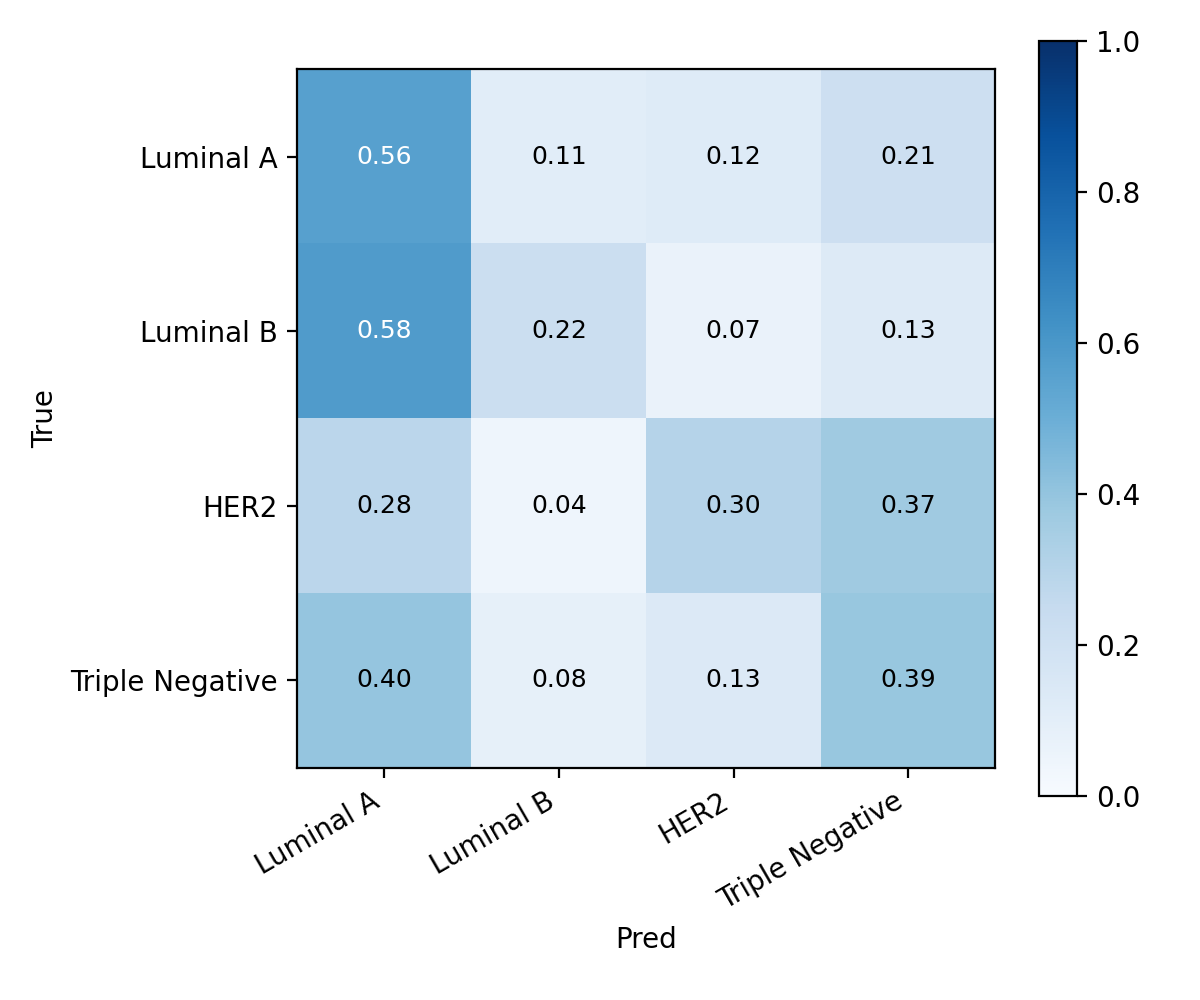
\includegraphics[width=0.72\linewidth]{figures/confusion_matrix.png}
  \caption{Normalised confusion matrix for the five-fold
    ensemble on the four-class centralised task.
    Each cell shows the fraction of true-class samples
    predicted as each class. Luminal~A achieves the
    strongest diagonal entry (0.56), while HER2 and
    Luminal~B show the most confusion with each other
    and with Luminal~A, reflecting the overlapping
    imaging phenotypes of hormone-receptor-positive
    subtypes.}
  \label{fig:confusion-matrix}
\end{figure}

\subsection{ROC Curves}
\label{sec:roc-curves}

\begin{figure}[htbp]
  \centering
  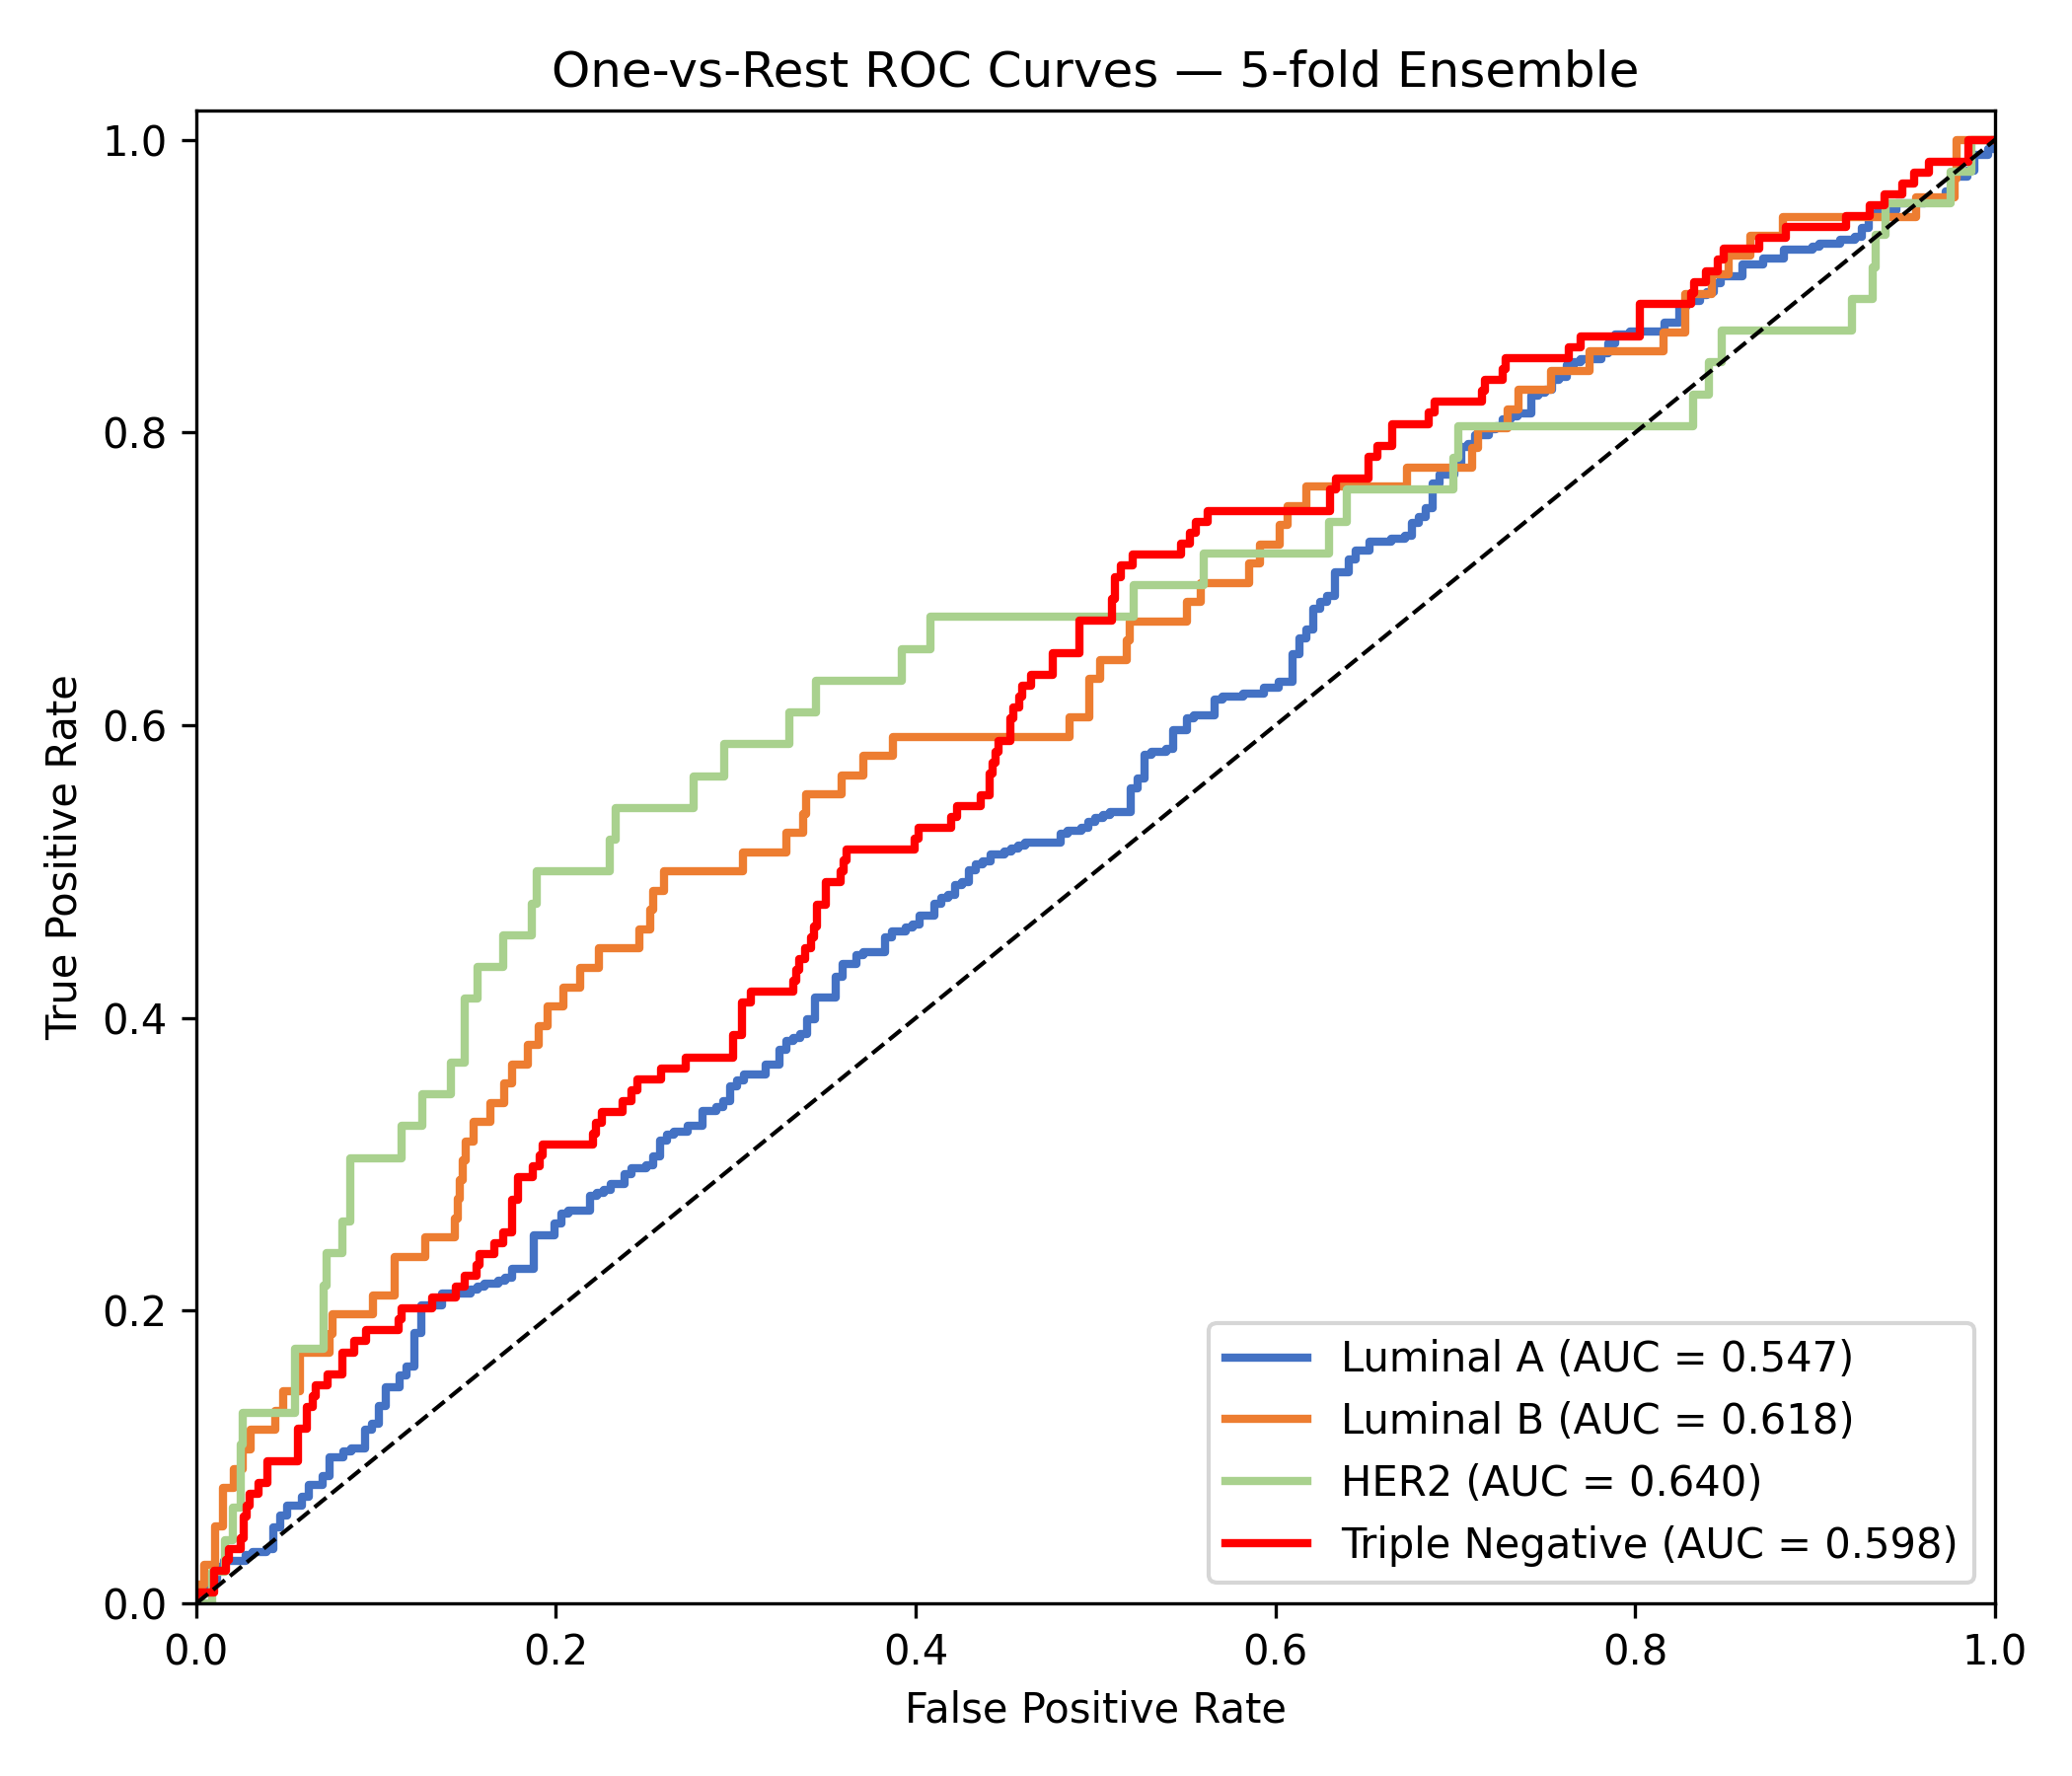
\includegraphics[width=0.78\linewidth]{figures/roc_curves.png}
  \caption{One-versus-rest ROC curves for each molecular
    subtype on the five-fold ensemble. The macro-averaged
    AUC-ROC of 0.601 confirms that the model has learned
    discriminative representations beyond random chance
    for all four subtypes. Luminal~A achieves the highest
    per-class AUC, consistent with its majority-class
    advantage, while HER2 achieves the lowest, reflecting
    the fundamental data scarcity of 46 training samples.}
  \label{fig:roc-curves}
\end{figure}

\subsection{Calibration Analysis}
\label{sec:calibration}

\begin{figure}[htbp]
  \centering
  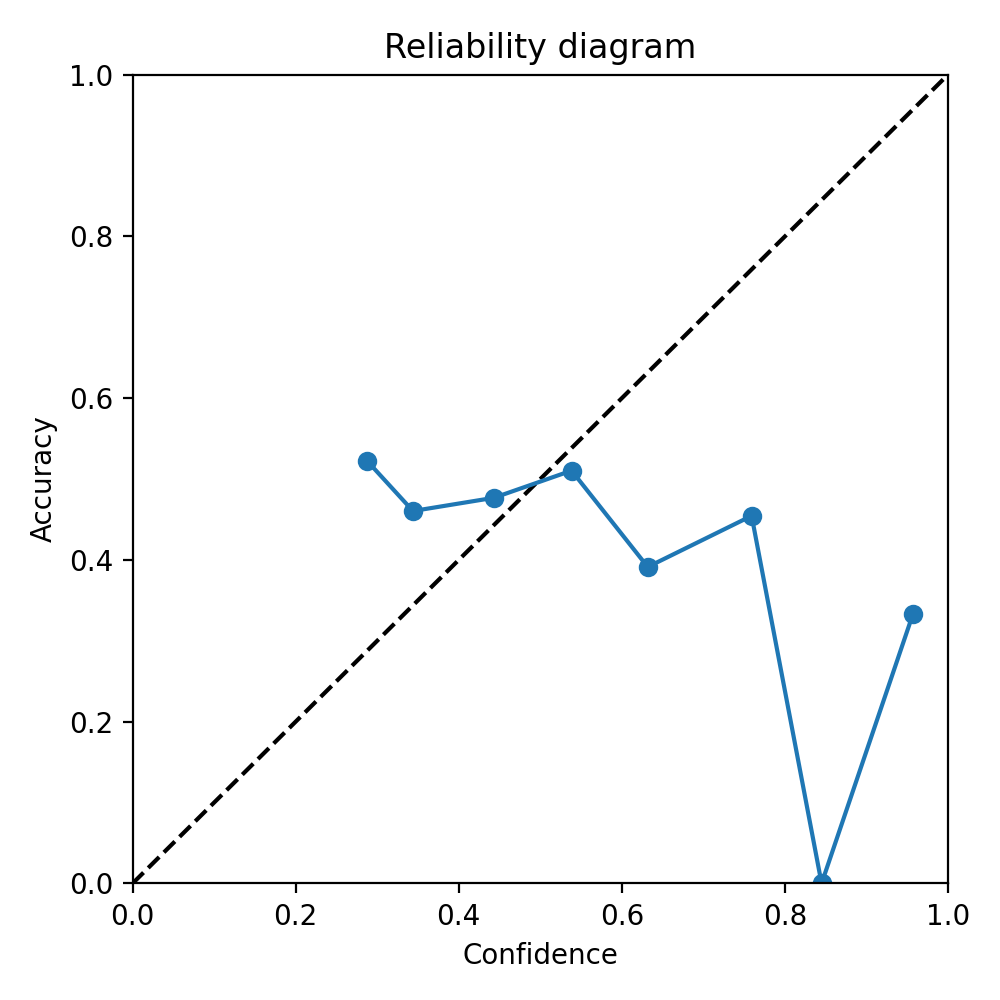
\includegraphics[width=0.60\linewidth]{figures/reliability.png}
  \caption{Reliability diagram for the five-fold ensemble.
    The diagonal dashed line represents perfect calibration.
    The model is overconfident at high confidence values,
    a known consequence of training with LDAM margin loss
    and class-imbalanced data where the majority class
    pushes softmax outputs toward high-confidence predictions.
    Brier score = 0.681.}
  \label{fig:reliability}
\end{figure}

\subsection{Radiomics Fusion}
\label{sec:results-fusion}

% TODO — insert fold-0 radiomics fusion result.
% Compare: deep features only vs deep + radiomics
% Expected gain: +0.04-0.06 F1


% ============================================================
\section{Comparison with State of the Art}
\label{sec:sota-comparison}
% ============================================================

Table~\ref{tab:sota} positions the centralised result within
the published literature on breast MRI molecular subtype
classification.
Direct numerical comparison is complicated by differences
in dataset, class definition, evaluation protocol, and
whether segmentation masks were used for region-of-interest
extraction.
All works listed below use variants of the Duke Hospital
dataset introduced by Saha~et~al.\ \cite{saha2018} or
comparable DCE-MRI cohorts.

\begin{table}[htbp]
  \centering
  \caption{Comparison with published results on breast
    MRI molecular subtype classification. The proposed
    method operates without tumour segmentation masks,
    a constraint not shared by most prior works.}
  \label{tab:sota}
  \renewcommand{\arraystretch}{1.3}
  \resizebox{\textwidth}{!}{%
  \begin{tabular}{llccc}
    \toprule
    \textbf{Method} & \textbf{Task}
      & \textbf{Segmentation?}
      & \textbf{Metric}
      & \textbf{Value} \\
    \midrule
    Saha et al.\ \cite{saha2018} & 4-class & Yes (ROI)
      & AUC & 0.65--0.70 \\
    Ghosh et al.\ \cite{ghosh2020clustered}
      & Various & Varies & F1 macro & $\sim$0.40--0.55 \\
    \textbf{Proposed (centralised)} & 4-class
      & \textbf{No} & \textbf{F1 macro} & \textbf{0.342} \\
    \textbf{Proposed (federated, FedAvg)}
      & Binary & No & F1 macro & TODO \\
    \textbf{Proposed (federated, SCAFFOLD)}
      & Binary & No & F1 macro & TODO \\
    \bottomrule
  \end{tabular}}
\end{table}

The proposed centralised result of $0.342$ macro F1 is
below the upper range of reported values in the literature.
This gap is explained by three factors specific to this
work.
First, no tumour segmentation mask is used; the model must
identify the discriminative enhancing region from the full
breast volume without spatial guidance, which is a strictly
harder task.
Second, the training set is limited to 737 patients,
whereas several published systems train on larger cohorts
or augment with external data.
Third, the evaluation uses a strict patient-level
stratified group split that prevents any patient from
appearing in both training and validation, eliminating
a common source of optimistic bias in prior works that
use random sample-level splits.
The primary contribution of this thesis is not to surpass
existing four-class results on this dataset, but to
quantify the federated privacy cost and the SCAFFOLD
convergence gain under realistic non-IID conditions
without segmentation masks.


% ============================================================
\section{Conclusion}
\label{sec:ch4-conclusion}
% ============================================================

This chapter has presented the implementation and results
of the centralised and federated experiments.
The centralised ConvNeXt-Nano plus Gated Attention MIL
pipeline achieves a five-fold macro F1 of $0.342$
(95\% CI: $[0.301, 0.382]$) on the four-class molecular
subtype task without tumour segmentation masks, establishing
a clear performance ceiling whose HER2 component ($F1 =
0.20$) confirms the fundamental data scarcity constraint
that motivates the binary federated reformulation.

% TODO — complete conclusion paragraph when FL results
% are available. Template:
% The binary federated experiment demonstrates that FedAvg
% achieves macro F1 of [X] versus the centralised binary
% baseline of [Y], a gap of [Z] points attributable to
% client drift under the non-IID Dirichlet partition.
% SCAFFOLD's control-variate correction recovers [W] of
% this gap, achieving macro F1 of [V] and confirming that
% convergence-aware aggregation is effective in cross-silo
% breast MRI federation with three hospital clients.

The General Conclusion synthesises both experiments and
identifies directions for future work.

% \chapter*{General Conclusion and Perspectives}
\addcontentsline{toc}{chapter}{General Conclusion and Perspectives}

% \include{Chapters/annexe}

\printbibliography
\end{document}